\documentclass[12pt, a5paper]{article}
\usepackage[utf8]{inputenc}
\usepackage[T2A]{fontenc}
\usepackage[russian]{babel}
\usepackage{amsmath}
\usepackage{amsfonts}
\usepackage{amssymb}
\usepackage[left=2cm,right=1cm,top=2cm,bottom=2cm, twoside]{geometry}
\usepackage{lscape}
\usepackage{comment}

\usepackage{pgf,tikz}
\usetikzlibrary{arrows}

\binoppenalty=10000
\relpenalty=10000	

\newcommand{\header}[2]
{
	\subsection{{#1}}
	\begin{center}
%	\textbf{#1}\\
	#2
	\end{center}
}

\sloppy

\graphicspath{{solutions/}}

%space from foothead
\headsep=12pt
\setlength{\headheight}{28pt} 

%header


%center sections name
\usepackage[explicit]{titlesec}
\titleformat{\section}{\normalfont\bfseries\center}{}{1em}{#1}
\titleformat{\subsection}{\normalfont\bfseries\center}{}{1em}{#1}


\renewpagestyle{headings}{
\sethead[\subsectiontitle][][]
{}{}{\sectiontitle}
\headrule
\setfoot[\thepage][][]
{}{}{\thepage}
}

\begin{document}

\begin{titlepage}
\begin{center}
\vfill

Московский государственный университет\\
имени М.В.~Ломоносова\\
Казахстанский филиал\\

\vfill

{\large\bf 
Студенческие олимпиады по математике\\
Казахстанского филиала МГУ.\\
Задачи и указания. \\
2008--2018 гг.\\}

\vfill

Астана\\
2018
\end{center}
\end{titlepage}

\setcounter{page}{2}


\thispagestyle{empty}

\noindent{\bf УДК} \\
{\bf ББК}\\
{\bf Л}
\vspace{0.7 cm}


{\bf ISBN}  

\vspace{0.7 cm}

В настоящем сборнике представлены более 100 задач студенческих олимпиад по математике Казахстанского филиала МГУ имени М.В.Ломоносова за период с 2008 по 2018 год.

Сборник  адресован  всем интересующимся олимпиадным движением.

\vspace{0.5 cm}

{\bf Составители:}

Абдикалыков А.К., Баев А.Ж., Васильев А.Н.

\vspace{0.5 cm}


{\bf TeX--верстка:}

Баев А.Ж.

\newpage
\begin{small}
\begin{center}
\textbf{Предисловие}
\end{center}
В Казахстанском филиале  МГУ имени М.В.~Ломоносова ежегодно проводятся студенческие олимпиады по математике. На базе Казахстанского филиала проводится также Республиканский этап студенческой предметной олимпиады по математике (2016 и 2017~гг.). Проведение олимпиады в Филиале (уже во второй раз) является результатом побед наших студентов на данной олимпиаде в предыдущие годы.

Ежегодно в декабре студенты Казахстанского филиала проходят отбор внутри университета для участия на Республиканском этапе. В связи со спецификой обучения в Филиале, на олимпиаде участвуют студенты первого и второго курсов механико--математического факультета и факультета вычислительной математики и кибернетики (студенты третьего и четвертого курса продолжают обучение в Москве). На олимпиаде обычно предлагается от 7 до 10 заданий по математическому анализу, алгебре, геометрии, теории чисел, дискретной математике и по крайней мере одна задача из коллекции школьных олимпиад по математике. Такой вариант позволяет первокурсникам свободно конкурировать со студентами второго курса. Победители справляются, как правило, с 4 или 5 заданиями.

В данном сборнике представлены тексты около 100 задач олимпиад последних десяти лет, к которым даны указания, составленные преподавателями Казахстанского филиала. При подготовке олимпиад использованы материалы из различных сборников студенческих и школьных олимпиад, а также авторские задачи. Авторами задач являются преподаватели филиала Абдикалыков А.К., Баев А.Ж., Васильев А.Н., которые активно участвуют в олимпиадном движении Казахстана. 

Составители выражают благодарность профессору  Нурсултанову~Е.Д. и доценту Бекмаганбетову~К.А. за оказание содействия при подготовке сборника.

\begin{flushright}
Директор Казахстанского филиала

А.В.Сидорович
\end{flushright}
\end{small}

\newpage

\mbox{}

\newpage
\pagestyle{headings}

\tableofcontents

\newpage

\section{Условия задач олимпиад Казахстанского филиала}

\header{2008--2009}{7 декабря 2008}
\begin{enumerate}
\item Функция $f(x)$ имеет непрерывную вторую производную, причем $f^{''}(x)>0$ при $x \in [0, 2\pi]$. Докажите, что  
$$ \int\limits_0^{2\pi} f(x)\cos x\,dx > 0. $$

\item Пусть $A$ --- конечное множество действительных чисел. Определите мощность множества определённых на $[0,1]$ и непрерывных на этом отрезке функций, принимающих на множестве рациональных чисел значения из множества $A$.

\item Бой подушками на бревне проводится на вылет. Всем участникам присваиваются порядковые номера. Очередность боев определяется по возрастанию номеров: первый бьётся со вторым, победитель этой пары --- с третьим, следующий победитель --- с четвёртым и т.д. В другой день эти же бойцы решили повторить матч по тем же правилам, но очерёдность боев установили по убыванию номеров. Докажите, что найдётся пара бойцов, встречавшаяся друг против друга на бревне дважды.

\item Найти все дифференцируемые $(n+1)$ раз на числовой прямой функции, для которых при любом вещественном $x$ выполняется соотношение
$$
f(x)=f(0)+\frac{x}{1!}\,f'(0)+\frac{x^2}{2!}\,f''(0)+\cdots$$
$$\cdots + \frac{x^n}{n!}\,f^{(n)}(0)+\frac{x^{n+1}}{(n+1)!}\,f^{(n+1)}(x).
$$

\item Функция $f$: $\mathbb{R} \rightarrow (-\infty, +\infty)$ всюду непрерывна. Известно, что
$$ \int\limits_{-\infty}^{+\infty} f(x)\,dx = 1. $$
Пусть $\alpha$ --- произвольное вещественное число из интервала $(0, 1)$, а $[a, b]$ --- отрезок минимальной длины, для которого
$$\int\limits_{a}^{b} f(x)\,dx = \alpha.$$ Докажите, что $f(a) = f(b)$.

\item Пусть $\{a_1, a_2, \hdots, a_n\}$ --- множество натуральных чисел такое, что $\prod\limits_{i=1}^n a_i$ имеет менее $n$ различных простых делителей. Докажите, что существует непустое подмножество $I$ множества $\{1, 2, \hdots, n\}$ такое, что $\sqrt{\prod\limits_{i \in I} a_i}$ --- целое число.

\item Обозначим $k$-е по счету простое число через $p_k$. Докажите, что для любого $n \geqslant 2$ множество $\{1, 2, \hdots, n\}$ можно разбить на 2 таких подмножества $A$ и $B$, что
$$1 \leqslant \frac{ \prod\limits_{i \in A}{p_i} }{ \prod\limits_{j \in B}{p_j} } \leqslant 2.$$

\item Построить функцию $f(x)$, всюду разрывную, кроме $0$, но дифференцируемую в нуле, причем $f'(0)=1$.

\item Можно ли произвольную функцию $f: \mathbb{R} \rightarrow \mathbb{R}$ разложить в сумму сюръективной функции $g: \mathbb{R} \rightarrow \mathbb{R}$ и инъективной функции $h: \mathbb{R} \rightarrow \mathbb{R}$?

\end{enumerate}
\newpage

\header{2009--2010}{6 декабря 2009}
\begin{enumerate}

\item На доске написано число $-1000000$ (минус миллион). За ход разрешается выбрать какие-нибудь два (или одно) числа и написать их сумму или произведение. Если выбрано одно число, то надо писать или его квадрат, или его удвоенное. Как за 12 таких ходов написать число ноль?

\item Малыш может съесть торт за 10 минут, банку варенья --- за 8 минут и выпить кастрюлю молока --- за 15 минут, а Карлсон может сделать это за 2, 3 и 4 минуты соответственно. За какое наименьшее время они могут вместе покончить с завтраком, состоящим из торта, банки варенья и кастрюли молока?

\item Касательная к гиперболе $y = \displaystyle\frac{1}{x}$ в точке $M$ отсекает от угла $x \geqslant 0$, $y \geqslant 0$ прямоугольный треугольник. Докажите, что:\\
а) точка $M$ --- середина гипотенузы этого треугольника;\\
б) его площадь не зависит от выбора точки $M$.

\item Дифференцируемые функции $f(x)$ и $g(x)$ определены на отрезке $[0, 1]$ таким образом, что:\\
a) $f(0)=f(1)=1$; \\
б) $2001\cdot f'(x) g(x) + 2009\cdot f(x) g'(x) \geqslant 0$ для всех $x \in [0, 1]$.\\
Докажите, что $g(1) \geqslant g(0)$.

\item Найдите сумму ряда
$$\sum_{n=1}^{\infty} \arctg \left( \frac{1}{n^2+n+1} \right).$$

\item Пусть $\{ q_k \}_{k=1}^{n}$ --- конечная последовательность чисел. Известно, что $q_k \geqslant 1$ для всех $k$. Докажите неравенство:
$$ \sqrt[q_1]{1 + \sqrt[q_2]{ 1 + \hdots + \sqrt[q_n]{1}}} \leqslant 1 + \frac{1}{q_1} + \frac{1}{q_1 q_2} + \hdots + \frac{1}{q_1 \hdots q_n}. $$

\item Найдите минимум величины $\max\limits_{1 \leqslant i < j \leqslant n+1} (x_i, x_j)$ по всем наборам единичных векторов $x_1$, $x_2$, ..., $x_{n+1} \in \mathbb{R}^n$.

\end{enumerate}

\newpage

\header{2010--2011}{12 декабря 2010}
\begin{enumerate}

\item Пусть функции $f(x)$, $g(x)$ --- непрерывные и сюръективные отображения из $[0, 1]$ в $[0, 1]$. Докажите, что найдётся точка $x_0$ из отрезка $[0, 1]$ такая, что $f(g(x_0)) = g(f(x_0))$.

\item Пусть $r \in\mathbb N$. Найти предел
$$\lim_{n \rightarrow \infty} \frac{1}{n^{r+1}} \sum_{k=1}^n k^r \cos \frac{k}{n}.$$

\item Пусть $\sum\limits_{n=1}^{\infty} a_n = S$. Доказать, что
$$\lim_{x \rightarrow 1 - 0} \left( a_1 + a_2 x + \hdots + a_n x^{n-1} + \hdots \right) = S.$$

\item Пусть $f$ есть (не обязательно дифференцируемая) функция, удовлетворяющая для любой пары $x_1 < x_2$ неравенству
$$ f \left( \frac{x_1 + x_2}{2} \right) < \frac{f(x_1) + f(x_2)}{2}.$$
Доказать, что тогда верно неравенство
$$ f \left( \frac{x_1 + x_2 + \hdots + x_n}{n} \right) < \frac{f(x_1) + f(x_2) + \hdots + f(x_n)}{n}.$$

\item У числа $a$ есть $p$ делителей, $p$ --- простое число. Докажите, что $a (a^k - 1)$ делится на $p$ для любого натурального $k$.

\item Существуют ли квадратные матрицы $A$, $B$ такие, что $AB - BA = E$, где $E$ --- единичная матрица?

\item Рассмотрим ряд $\sum\limits_{n=1}^{\infty} \frac{\cos{n}}{n}$. Разобьем $N$-ю частичную сумму этого ряда на два слагаемых:
$$ S_N = \sum_{n=1}^{N} \frac{\cos{n}}{n} = S_N^{+} + S_N^{-},$$
где $S_N^{+}$ и $S_N^{-}$ --- суммы соответственно положительных и отрицательных членов. Докажите, что существует предел $\lim\limits_{N \rightarrow \infty}{\frac{S_N^{+}}{S_N^{-}}}$ и найдите его.

\item Дано конечное множество точек $\Delta = \{ A_1, A_2, \hdots, A_n \}$ на плоскости и положительное число $\rho > 0$. Для произвольной точки $X$ плоскости построим последовательность точек $\{X_k\}_{k=1}^{\infty}$ по следующему правилу: $X_1 = X$, $X_{k+1}$ --- это центр тяжести точек из $\Delta$, содержащихся в круге радиуса $\rho$ с центром в точке $X_k$, если такие точки существуют, и $X_{k+1} = X_k$ иначе. Докажите, что при любом выборе начальной точки $X$ данная последовательность будет постоянной, начиная с некоторого номера.

\end{enumerate}
\newpage

\header{2011--2012}{10 декабря 2011}
\begin{enumerate}
\item Назовем конечное числовое множество своеобразным, если оно содержит число, равное количеству его элементов, но никакое его собственное подмножество этим свойством не обладает. Определите количество своеобразных подмножеств множества $\{1,\;2,\;\dots,\;12\}$.

\item Определите множество значений функции, сопоставляющей каждому прямоугольному треугольнику отношение~$\displaystyle\frac{h}{r}$, где $h$ --- высота, проведенная к гипотенузе, а $r$~---~радиус вписанной в треугольник окружности.

\item Две последовательности $\{x_n\}_{n=0}^{\infty}$ и $\{y_n\}_{n=0}^\infty$ удовлетворяют условиям:
$$
\begin{cases}
x_{n+1}=2x_n-\alpha y_n,\\
y_{n+1}=2y_n-\displaystyle\frac{1}{\alpha} x_n
\end{cases}
$$
при всех $n\geqslant 0$, где $\alpha\not=0$ --- постоянная величина, а $x_0=1$ и $y_0=0$. Найдите $x_{2012}$ и $y_{2012}$.

\item Существует ли такая последовательность вещественных чисел $\{x_n\}_{n=1}^{\infty}$, что для неё справедливы соотношения: \begin{equation*}
\left\{
\begin{aligned}
\lim\limits_{k\to\infty}x_{12k} = 20,\\
\lim\limits_{k\to\infty}x_{20k} = 12?\\
\end{aligned}
\right.
\end{equation*}

\item Найдите $\displaystyle\int\limits_{0}^{\pi/2}\left(\sin^2(\sin^2x)+\cos^2(\cos^2x)\right)\,dx$.

\item Найдите $\displaystyle\sum\limits_{n=0}^{\infty}\frac{n+2}{n!+(n+1)!+(n+2)!}$.

\item Найдите все функции $f\colon[0,\;1]\to \mathbb R$, удовлетворяющие неравенству $(x-y)^2\leqslant |f(x)-f(y)|\leqslant|x-y|$ для любых $x, y\in[0,\;1]$.

\item Пусть $x_1,\;x_2,\;\dots,\;x_n,\;\dots$ --- все положительные корни уравнения $\mathrm{tg}\,x=x$, выписанные в порядке возрастания, $n_1,\;n_2,\;\dots,\;n_k,\;\dots$ --- некоторая возрастающая последовательность натуральных чисел. Докажите, что ряды $\displaystyle\sum\limits_{k=1}^{\infty} |\cos x_{n_k}|$ и $\displaystyle\sum\limits_{k=1}^{\infty}\frac{1}{n_k}$ сходятся или расходятся одновременно.

\item Квадратная матрица $A$ порядка $n$ состоит из чисел $+1$ и $-1$. При этом, в каждой строке и в каждом столбце этой матрицы находится ровно одно число $-1$. Найдите $|\det A|$.

\item Пусть $S$ --- сумма всех обратимых элементов конечного ассоциативного кольца с единицей. Докажите, что $S^2=0$ или $S^2=S$.
\end{enumerate}

\newpage

\header{2012--2013}{21 декабря 2012}
\begin{enumerate}

\item Будем называть целочисленную квадратную матрицу порядка $n$ <<весёлой>>, если сумма элементов каждой её строки чётна. Докажите, что для любой целочисленной матрицы $A$ и для любой <<весёлой>> матрицы $B$ произведение $AB$ тоже является <<весёлой>> матрицей.

\item  Пусть ($A$, $+$, $*$) --- конечное кольцо с единицей, в котором $1 + 1 = 0$. Докажите, что уравнения
$x^2 = 0$ и $x^2 = 1$ имеют одинаковое количество корней в кольце.

\item Прямые $l_1$ и $l_2$ касаются параболы в точках $A$ и $B$, соответственно, и пересекаются в точке $C$. Точка $K$ --- середина отрезка $AB$. Докажите,что середина отрезка $KC$ лежит на параболе.

\item При каких натуральных $n$ выполняется равенство
$$\sum\limits_{k=1}^n \left[ \sqrt[k]{n}\,\right] = 2 n ?$$

\item Последовательность 1, 3, 4, 9, 10, 12, 13, $\hdots$ состоит из всех натуральных чисел, являющихся степенью 3 или представимых в виде суммы различных степеней 3. Найдите 100-й член этой последовательности.

\item Квадратная матрица $A$ порядка $m$ такова, что $A^{n+1} = 0$, а $A^n$ не равна нулевой. Докажите, что 
$$a_n A^n + a_{n-1} A^{n-1} + \hdots + a_1 A + a_0 E = 0$$
тогда, и только тогда, когда вещественные коэффициенты $a_i = 0$ при любом $i = 0, 1, \hdots, n$. Здесь $E$ --- единичная матрица.

\item Вычислите сумму ряда
$$\sum_{k=1}^{\infty} \frac{1}{1^3 + 2^3 + \hdots + k^3}.$$
Примечание: соотношение $\zeta(2) = \sum\limits_{n=1}^{\infty} \frac{1}{n^2} = \frac{\pi^2}{6}$ считать известным.

\item Докажите, что 11 коней не могут побить все оставшиеся 53 поля шахматной доски.

\item Пусть $f: [0, 1] \rightarrow \mathbb{R}$ --- непрерывная функция, для которой $\int\limits_{0}^{1} x f(x)\,dx = 0$. Докажите, что
$$\int\limits_{0}^{1} f^2(x)\,dx \geqslant 4 \left( \int\limits_{0}^{1} f(x)\,dx \right)^2.$$


\end{enumerate}


\newpage

\header{2013--2014}{20 декабря 2013}
\begin{enumerate}
\item Можно ли разрезать квадрат 7$\times$7 на 5 частей так, чтобы из них можно было сложить 3 квадрата попарно различных целых площадей?

\item Известно, что $a$, $b$ и $c$ --- корни уравнения $x^3 + px + q = 0$. Вычислите определитель матрицы:
\begin{equation*}
\begin{pmatrix}
a & b & c\\
c & a & b\\
b & c & a\\
\end{pmatrix}.
\end{equation*}

\item На плоскости дана парабола. Найдите множество точек плоскости, из которых парабола видна под прямым углом (т.е. касательные, проведённые из этой точки, перпендикулярны друг другу).

\item Бинарная операция $*$: $\mathbb{R} \times \mathbb{R} \rightarrow \mathbb{R}$ удовлетворяет соотношению $(a * b) * c = a + b + c$ для любых вещественных чисел $a$, $b$ и $c$. Докажите, что $a * b = a + b$ для любых вещественных $a$ и $b$.

\item Назовем перестановку чисел от $1$ до $N$ <<интересной>>, если никакое число не стоит на своем месте ($a_i \ne i$). Обозначим $S(N)$ количество <<интересных>> перестановок чисел от $1$ до $N$. Вычислите:\\
a) $S(N)$;\\
б) $\lim\limits_{N \rightarrow \infty} \frac{S(N)}{N!}$.

\item Определите все вещественные числа $k$, для которых справедливо соотношение:
$$\int\limits_{1}^{2} \left( 1 + k \ln{x} \right) x^{x^k + k - 1} dx = 15.$$

\item Докажите, что:\\
a) существует бесконечно много целых чисел, не представимых в виде суммы кубов трёх целых чисел (среди которых могут быть равные);\\
б) любое целое число представимо в виде суммы кубов пяти целых чисел (среди которых могут быть равные).

\item Пусть $n$ --- натуральное число, кратное 4. Посчитайте количество различных биекций $f: \{1, \hdots, n\} \rightarrow \{1, \hdots, n\}$ таких, что $f(j) + f^{-1}(j) = n + 1$ для всех $j = 1, \hdots, n$. 

Пример: для биекции $f: (1, 2, 3, 4) \rightarrow (2, 4, 1, 3)$ обратной будет $f^{-1}: (1,2,3,4) \rightarrow (3, 1, 4, 2)$.

\item Известно, что $P(x)$ --- многочлен степени $n$ такой, что для всех $t \in \{ 1, 2, 2^2, \hdots, 2^n \}$ верно $P(t) = \frac{1}{t}$. Найдите $P(0)$.

\item В графе $G$ все вершины степени $k$. При этом в $G$ нет треугольников и для любых двух вершин, у которых нет общего ребра, найдутся ровно две вершины, с которыми есть общие рёбра у каждой из этих двух вершин. Чему равно количество вершин $G$?

\end{enumerate}

\newpage

\header{2013--2014 (дополнительный тур)}{15 марта 2014}
\begin{enumerate}

\item Вычислить произведение двух чисел с помощью операций сложения, вычитания, возведения в квадрат и взятия обратного числа. Возможностью обращения знаменателя в 0 пренебречь.

\item Пусть $\alpha$, $\beta$, $\gamma$ --- три различных корня уравнения $$x^3 - x - 1 = 0.$$ 
Вычислите:
$$\frac{1-\alpha}{1+\alpha} + \frac{1-\beta}{1+\beta} + \frac{1-\gamma}{1+\gamma}.$$

\item Найти максимальное значение определителя третьего порядка, у которого 2 элемента равны 4, а остальные 1 или -1.

\item Решите в комплексных числах систему:
\begin{equation*}
\begin{cases}
\sqrt{3} z^{11} - z^{10} - 1 = 0 \\
|z| = 1
\end{cases}
\end{equation*}

\item Вычислите интеграл
$$\int\limits_{-1}^{1} \frac{dx}{(e^x + 1)(x^2 + 1)} .$$

\item Из точки $P$ к параболе с фокусом $F$ провели две касательные $PX$ и $PY$. Докажите, что:
$$FP^2 = FX \cdot FY .$$

\item Обозначим $f(x) = a x^2 + b x + c$, $a > 0$. Известно, что уравнение $f(x) = x$ не имеет решений. Докажите, что последовательность $a_n = \min \underbrace{f(f( \cdots f}_{n} (x) { \cdots ))} $ --- возрастающая.

\item Даны натуральные числа $m$, $n$ такие, что $m^2 - 2 n^2 = 1$, и даны функции: 
\begin{equation*}
\begin{aligned}
f_1(x) &= \cos(x),\\
f_2(x) &= \ctg(x),\\
f_3(x) &= \arctg(x). 
\end{aligned}
\end{equation*}
Докажите, что существует композиция $H(x)$ из указанных функций (некоторые функции могут быть использованы несколько раз, а некоторые ни разу) такая, что $H(1) = \frac{m}{n}$.

\item Пусть $p_1 = 2$, $p_2 = 3$, $p_3 = 5$, ..., $p_n$ --- возрастающая последовательность всех простых чисел, не превосходящих~$2^{100}$. Докажите, что:
$$\frac{1}{p_1} + \frac{1}{p_2} + ... + \frac{1}{p_n} < 10 .$$

\end{enumerate}


\newpage

\header{2014--2015}{10 декабря 2014}
\begin{enumerate}
\item Найдите все непрерывные функции $f: \mathbb{R} \rightarrow \mathbb{R}$, удовлетворяющие уравнению

$$ 3 f(2 x + 1) = f( x ) + 5 x.$$

\item Известно, что

$$ \int\limits_{0}^{1} \frac{\ln(1+x)}{x}\,dx = \frac{\pi^2}{12}.$$

Вычислите

$$ \int\limits_{0}^{1} \frac{\ln(1-x^3)}{x}\,dx.$$

\item Пусть $\{ \varepsilon_n \}_{n=1}^{\infty}$ --- последовательность, состоящая из чисел $1$ и $-1$. Может ли число

$$\sum_{n=1}^{\infty} \frac{\varepsilon_n}{n!}$$

быть рациональным?

\item Для квадратных матриц одного порядка $A$ и $B$ верно $AB = A + 2014B$. Докажите, что сумма коэффициентов характеристического многочлена матрицы $B$ не равна нулю.

\item Двое играют в игру. На доске написано число $n$. За один ход разрешается уменьшить число на любой из его целых положительных делителей (в том числе на единицу или на само это число). Если при этом получается нуль, игрок проиграл. Ходы делаются поочерёдно. Какой из двух игроков выиграет, если они оба играют оптимально?

\item Дано вещественное число $x$ такое, что $x^3 = x + 1$. Доказать, что $x^5 = x^4 + 1$.

\item  Найти сумму ряда

$$\sum_{n=1}^{\infty} {\mathrm{arcctg}}~{F_{2n+1}}, $$
где $F_n$ --- числа Фибоначчи ($F_1=F_2=1$, $F_{n+2} = F_{n+1}+F_n$ для $n\in\mathbb N$).

\item Пусть $a_n$ --- число обратных самих себе перестановок порядка $n$. Доказать $a_{n+1} = a_n + n a_{n-1}$.

\item Прямоугольник размером $N \times M$ ($N>2$, $M>2$) разбит равномерной сеткой на $N M$ квадратов $1 \times 1$. Назовем его красивым, если все клетки $1 \times 1$ можно покрасить в один из двух цветов так, чтобы никакие 4 клетки, образующие прямоугольник со сторонами, параллельными сторонам исходного прямоугольника, не были покрашены в один цвет. Найдите красивый прямоугольник максимальной площади.

\item Докажите, что ортоцентр треугольника, описанного около параболы, лежит на её директрисе.
 
\end{enumerate}
\newpage

\header{2015--2016}{19 декабря 2015}
\begin{enumerate}

\item $a_n$, $b_n$, $x_n$, $y_n$ --- четыре арифметические прогрессии. Известно, что $a_n b_n = x_n y_n$ для трёх различных натуральных $n$. Доказать, что $a_n b_n = x_n y_n$ для всех натуральных $n$.

\item Пусть $f(n)$ --- вещественнозначная функция, определённая на множестве натуральных чисел и удовлетворяющая следующему условию: для любого $n > 1$ существует такой его простой делитель $p$, что $f(n) = f\left( \frac{n}{p} \right) - f(p)$. Известно, что $f(2015) = 2015$. Найдите $f(2016)$.

\item Найдите все дифференцируемые функции $f: \mathbb{R} \rightarrow \mathbb{R}$, удовлетворяющие следующим двум условиям:\\
а) $f'(x) = 0$ для всех $x \in \mathbb{Z}$;\\
б) если для некоторого $x_0 \in \mathbb{R}$ справедливо равенство $f'(x_0) = 0$, то для него справедливо также равенство $f(x_0) = 0$.

\item На параболе выбраны 4 точки: $A_1$, $A_2$, $A_3$ и $A_4$. Через эти точки к параболе проведены 4 касательные $l_1$, $l_2$, $l_3$ и $l_4$ соответственно. $l_1$ пересекает $l_2$ в точке $M$. $l_3$ пересекает $l_4$ в точке $N$. Докажите, что $MN$, $A_1A_3$ и $A_2A_4$ пересекаются в одной точке.

\item Решить в вещественных числах уравнение
$$4x + 2 \sin{x} + \sin( 2x + \sin{x} ) + 12 \pi = 0.$$

\item Дано $n$ натуральных чисел $a_1$, $a_2$, $\hdots$, $a_n$, при этом все они не превосходят $n$. Доказать, что существует непустое подмножество $P = \{p_1, \hdots, p_k \}$ множества $\{1, 2, \hdots, n\}$ такое, что множества $P$ и $\{ a_{p_1}, a_{p_2}, \hdots, a_{p_n} \}$ совпадают.

\item Найдите все матрицы $A$, которые обладают следующими свойствами:\\
а) имеет всего одно собственное значение (без учёта кратности);\\
б) ранг равен 1;\\
в) след равен 1.

\end{enumerate}
\newpage

\header{2016--2017}{10 декабря 2016}
\begin{enumerate}
\item Докажите, что для любого натурального $n$ верно равенство:
$$\int\limits_0^{2\pi} {\sin(\sin x + nx)}~dx = 0.$$

\item Существует ли такой многочлен $P(x)$, что $P(1) = 2$, $P(2) = 1$ и $P(x)$ принимает иррациональные значения для всех рациональных $x$, кроме 1 и 2? 

\item Для положительных чисел $a_i$ известно, что 
$$a_1 \cdot a_2 \cdot \ldots \cdot a_n = 1.$$ 
Докажите, что функция 
$$f(x) = (1 + a_1^x)(1 + a_2^x) \dots (1 + a_n^x)$$
неубывающая при $x > 0$.

\item Дан тетраэдр, грани которого имеют одинаковую площадь. Докажите, что все его грани равны.

\item Для набора вещественных чисел $c_0, c_1, \dots, c_n$ известно, что 
$$c_0 + \frac{c_1}{2} + \frac{c_2}{3} + \ldots + \frac{c_n}{n+1} = 0.$$
Докажите, что уравнение $c_0 + c_1 x + c_2 x^2 + \ldots + c_n x^n = 0$ имеет хотя бы один вещественный корень. 

\item $A$ --- ассоциативное кольцо с единицей (не гарантируется, что умножение коммутативно). $D$ --- множество всех необратимых элементов $A$. Известно, что $a^2 = 0$ для всех элементов $a \in D$. Докажите, что $axa = 0$ для всех $a \in D$, $x \in A$.

\item Дана матрица $A$ размером $n \times n$, где элементы матрицы $a_{ij}$ равны последней цифре числа $(i+j-2)$. 
\begin{enumerate}
\item Вычислите определитель матрицы при $n \leqslant 8$;
\item Вычислите определитель матрицы при $n \geqslant 11$;
\item Докажите, что определитель матрицы делится на $10^7$ при $n = 9$ и $n = 10$.
\end{enumerate}

\item Обозначим частичную сумму гармонического ряда через 
$$H_n = \frac{1}{1} + \frac{1}{2} + \frac{1}{3} + \ldots + \frac{1}{n}.$$ 
Найти сумму следующего ряда:
$$\frac{H_1}{10} + \frac{H_2}{100} + \frac{H_3}{1000} + \ldots$$
\end{enumerate}
\newpage

\header{2017--2018}{9 декабря 2017}
\begin{enumerate}
\item Привести пример вещественной матрицы $A$ такой, что $A^4 = I$, но при этом $A^2 \neq \pm I$, где $I$ --- единичная матрица.

\item Существует ли такая расходящаяся числовая последовательность $\{x_n\}$, что при любом натуральном $k > 1$ её подпоследовательность $\{x_{kn}\}$ сходится?

\item Вычислите
$$
\int\limits_{-1}^{1} \frac{x^{2k} + 2017}{2018^x + 1} \;dx ,
$$
где $k\in\mathbb Z$.

\item Найдите все непрерывные функции $f: \mathbb{R} \to \mathbb{R}$ такие, что 
$$f(x) + f\left(3 - \frac{9}{x}\right) = x - \frac{9}{x}$$
для всех $x\in\mathbb R\setminus\{0, 3\}.$

\item К параболе проведены две касательные $l_a$ и $l_b$ в точках $A$ и $B$. Точка $C$ симметрична точке $A$ относительно $l_b$, а точка $D$ симметрична точке $B$ относительно $l_a$. Докажите, что точки $A$, $B$, $C$ и $D$ образуют ромб тогда и только тогда, когда $AB$ проходит через фокус параболы.

\textit{Можно использовать оптическое свойство параболы без доказательства.}

\item Найдите все такие натуральные $n$, при которых 
$$C_{n}^0 \cdot C_{n}^1 \cdot \hdots \cdot C_n^n$$
является точным квадратом.

\textit{Здесь $C_n^k = \dfrac{n!}{k!(n-k)!}$ --- биномиальный коэффициент.}

\item Докажите сходимость последовательности $\{a_n\}$, где 
$$
\begin{cases}
a_1 = 1,\\
a_{n+1} = a_n + \sin{a_n},\\
\end{cases}
$$
и найдите её предел.

\item Функция $F(n, k)$, определённая для всех целых неотрицательных $n$ и $k$, удовлетворяет условиям
$$
\begin{cases}
F(n, k) = F(n - 1, k) + F(n, k - 1), & n \geqslant 1, k \geqslant 1,\\
F(n, 0) = 1,  & n \geqslant 0,\\
F(0, k) = 2 F(0, k - 1) + 1, & k \geqslant 1.
\end{cases}
$$
Вычислите $F(n, n)$.
\end{enumerate}
\newpage

\header{2017--2018 (дополнительный тур)}{13 марта 2018}
\begin{enumerate}
\item Найдите определитель матрицы $A$ порядка $n$, где 
$$a_{i j} = \frac{(i+j-2)!}{(i-1)! (j-1)!}$$
для всех $1 \leqslant i \leqslant n$ и $1 \leqslant j \leqslant n$.

\item Найдите сумму ряда
$$\sum_{i=2}^{\infty} \frac{3n^2 - 1}{(n^3 - n)^2}.$$

\item Найдите все непрерывные функции $f(x) : \mathbb{R} \to \mathbb{R}$ такие, что 
$$f(x^2) + f(x) = 2.$$

\item При каких $m$, $n$ правильный $m$-угольник можно разрезать на несколько (два и более) равных правильных $n$-угольников?

\item Дана обратимая выпуклая вниз функция $f(x) \in C(R)$. Известно, что существует такая точка $c$, что $f(c) < c$ и $f'(c) = 1$. Докажите, что существуют такие различные точки $a$ и $b$, что
$$\int\limits_{a}^{b} \left(f(x) + f^{-1}(x)\right) dx = b^2 - a^2.$$

\end{enumerate}
\newpage

\header{Республиканская олимпиада по математике 2016}{01 апреля 2016}
\begin{enumerate}

\item Какие натуральные числа представимы в виде $$x^2-y^2+2x+2y$$ для некоторых целых $x$ и $y$?

\item Пусть  $\alpha(x)$ --- первая цифра после запятой в десятичной записи числа $2^x$.\\
а) Докажите, что функция $\alpha(x)$ интегрируема по Риману на $[0, 1]$.\\
б) Докажите, что $\displaystyle 3.5 < \int\limits_{0}^{1} \alpha(x) dx < 4.5$.

\item В конечном поле произведение всех ненулевых элементов не равно единице. Докажите, что сумма всех элементов поля равна нулю.

\item В эллипсе с фокусами $F_1$ и $F_2$ проведена хорда $MN$, которая проходит через фокус $F_2$. На прямой $F_1F_2$ выбраны две точки $S$ и $T$ такие, что прямые $SM$ и $TN$ являются касательными к эллипсу. Точка $D$ симметрична $F_2$ относительно прямой $SM$, точка $E$ симметрична $F_2$ относительно $NT$. Прямые $DS$, $TE$ и $MN$ при пересечении образуют треугольник $ABC$ (точка $C$ не лежит на $MN$). Докажите, что:
\begin{itemize}
\item[а)] $CF_2$ --- медиана треугольника $ABC$;
\item[б)] $CF_1$ --- биссектриса треугольника $ABC$.
\end{itemize}

\item Максималист и минималист по очереди вписывают по одному числу в таблицу размера $n \times n$ (последовательно, строчка за строчкой, слева направо и сверху вниз). Каким окажется ранг получившейся матрицы, если максималист изо всех сил старается его максимизировать, а минималист --- минимизировать? (Ответ может зависеть от $n$ и от того, кто делает первый ход.) 
 
\item Функция $f : (1, +\infty) \rightarrow \mathbb{R}$ дифференцируема на всей области определения. Известно, что  $$\displaystyle f'(x) = f\left( \frac{x}{x-1} \right) + f(x)$$ для всех $x > 1$ и $\displaystyle \lim\limits_{x \to \infty} \frac{f'(x)}{e^x} = 2$. Докажите, что $f(2) < 20,\hspace{-2pt}16$.

\end{enumerate}

\newpage

\header{Республиканская олимпиада по МКМ 2016}{01 апреля 2016}
\begin{flushright}
Стоимость задач: \\
10 баллов каждая задача.\\
\end{flushright}

\begin{enumerate}
\item Введём функцию
$$
f(n) = \bigl[\sqrt 1\,\bigr] + \bigl[\sqrt 2\,\bigr] + \bigl[\sqrt 3\,\bigr] + \hdots + \bigl[\sqrt{n^2-1}\,\bigr] + \bigl[\sqrt{n^2}\,\bigr],
$$
где $[x]$ --- наибольшее целое число, не превышающее $x$. Опишите функцию, которая вычисляет $f(n)$ для данного натурального $n$, не используя при этом операцию извлечения корня и вещественную арифметику.

\item На декартовой координатной плоскости нарисованы две полупараболы: график функции $y = x^2$ $(x \geqslant 0)$ и его копия, повёрнутая на прямой угол по часовой стрелке. Эти две кривые отсекают от прямой, параллельной оси ординат, отрезок длины $L$. Обозначим через $S(L)$ --- площадь отсечённой фигуры.

a) Докажите, что $S(L) > 1$ при $L > 2$;

б) Напишите функцию, которая вычисляет $S(L)$ для данного положительного вещественного числа $L$.



\item Найдите все дифференцируемые функции $f\colon \mathbb R\rightarrow\mathbb R$, удовлетворяющие соотношению
$$
f(x-y) + f(x+y) = f'(x^2 + y^2)
$$
для любых $x,y\in\mathbb R$.



\item  Дана функция $f\colon [0, 2n]\rightarrow\mathbb R$. Пусть $f_i = f(i)$ --- значения функции во всех целых $i$ от 0 до $2n$. Дана переменная $S$ вещественного типа с начальным значением 0. За один ход робот может выбрать целое $i$ от 1 до $2n-1$, затем добавить к переменной $S$ или вычесть из нее среднее арифметическое значений функции $f(x)$ в узлах~$i-1$,~$i$,~$i+1$:
$$S := S \pm \frac{f_{i-1}+f_i+f_{i+1}}{3}.$$ 
Может ли робот за конечное число ходов получить в переменной $S$ значение
$$I = \frac{1}{3} \left(f_0 + 4\sum\limits_{k=1}^{n}{f_{2k-1}} + 2\sum\limits_{k=1}^{n-1}{f_{2k}} + f_{2n}\right),$$
которое является приближением интеграла $\displaystyle \int\limits_0^{2n} f(x)\,dx$, если\\
а) $f(0) = f(2n) = 0$;\\
б) $f(0) \ne 0$, $f(2n) \ne 0$?

\item  Дана некоторая условная машина, состоящая из памяти в $n$ бит и указателя, который в каждый отдельный момент находится над какой-то из этих n ячеек. Перед запуском программы в память записывается некоторое натуральное число $m$ в двоичной системе счисления, а указатель устанавливается над крайним правым (младшим) битом числа. Язык программирования для этой машины состоит из следующих команд:

\begin{center}
\begin{tabular}{|c|c|p{14cm}|}
\hline
{\bf L} & left & сместить указатель налево на одну ячейку, если это возможно, иначе завершить программу\\
\hline
{\bf R} & right & сместить указатель направо на одну ячейку, если это возможно, иначе завершить программу\\
\hline
{\bf C} & change & изменить значение бита в текущей ячейке на противоположное\\
\hline
{\bf A} & again & перейти к выполнению первой команды\\
\hline
{\bf S} & skip & пропустить две следующие команды, если в текущей ячейке 0\\
\hline
{\bf F} & finish & завершить выполнение программы\\
\hline
\end{tabular}
\end{center}

Команды записываются в одну строку и выполняются в последовательном порядке, слева направо. При этом запись программы обязана оканчиваться командой \textbf{A} или \textbf{F}. Напишите для этой абстрактной машины следующие программы:

а) заменить данное число на $(m - 1)$;

б) заменить данное число на $(2^n - m - 1)$;

в) изменить на противоположный его старший (крайний слева) бит.

\textit{Примеры:}

а) программа, обнуляющая все ячейки: \textbf{SSCLA};

б) программа, которая изменяет второй справа бит, если крайний справа бит нулевой: \textbf{SFFLCF}.


\item Из квадратной однородной пластины со стороной 1 случайным образом вырезается квадрат со сторонами, равными $2a$ и параллельными сторонам исходного квадрата. При этом центр квадрата --- это случайная величина, равномерно распределённая по всем допустимым положениям (квадрат со стороной $(1 - 2a)$).

a) Найдите вероятность $p(a)$ того, что центр тяжести полученной фигуры лежит в вырезанной области.

б) Опишите функцию $p(a)$, которая вычисляет указанную вероятность приблизительно, считая при этом, что нам не известен метод нахождения центра тяжести произвольной фигуры, однако мы можем найти центр тяжести конечного множества точек одинаковой массы.

\end{enumerate}

\newpage

\header{Республиканская олимпиада по математике 2017}{13 апреля 2017}
\begin{enumerate}

\item Пусть $(T_n)_{n=1}^{\infty}$ --- последовательность натуральных чисел, заданная рекуррентно: $T_1 = T_2 = T_3 = 1$ и $T_{n+3} = T_{n+2} + T_{n+1} + T_n$ при $n \geqslant 1$. Вычислите сумму ряда $$\displaystyle \sum\limits_{n=1}^{\infty} \frac{T_n}{2^n},$$
если известно, что данный ряд сходится.

\item Найдите все простые $p$, запись которых в $k$-ичной системе счисления при некотором натуральном $k > 1$ содержит ровно $k$ различных цифр (старшая цифра не может быть нулём).

\item Докажите, что в любой группе квадрат произведения двух элементов порядка два и куб произведения двух элементов порядка три всегда являются коммутаторами.

\item Точка $P$ лежит внутри выпуклой области, ограниченной параболой $y = x^2$, но не лежит на оси $OY$. Обозначим через $S(P)$ множество всех точек, полученных отражением $P$ относительно всех касательных к параболе.

а) Докажите, что значение суммы 
$$\displaystyle\max_{(x, y) \in S(P)} y ~ + \min_{(x, y) \in S(P)} y$$ не зависит от выбора точки $P$.

б) Найдите геометрическое место точек $P$ таких, что $\displaystyle\max_{(x, y) \in S(P)} y = 0.$

\item Для каждой функции $f: [0, 1] \to \mathbb{R}$ обозначим через $s_n(f)$ и $S_n(f)$ нижнюю и верхнюю суммы Дарбу для функции $f$, соответствующие равномерному разбиению $[0, 1]$ на $n$ частей. Существует ли такая интегрируемая функция $f$, что $\displaystyle \sum_{n=1}^{\infty} s_n(f)$ сходится, а
$\displaystyle\sum_{n=1}^{\infty} S_n(f)$ расходится?

\item Некоторые участники математической олимпиады списали решения некоторых задач у своих товарищей. Докажите, что можно с позором выгнать часть участников так, чтобы получилось, что более четверти от общего числа списанных решений было списано выгнанными участниками у не выгнанных.

\end{enumerate}

\newpage

\mbox{}

\newpage

\section{Указания}

\header{2008--2009}{7 декабря 2008}
\begin{enumerate}
\item С помощью интегрирования по частям докажите, что:

$$ \int\limits_0^{2\pi} f(x)\cos x\,dx = 
 \int\limits_0^{\pi} (f'(x+\pi) - f'(x)) \sin{x}\,dx. $$

\item Ответ: мощность конечна и совпадает с количеством элементов в $A$. Любая такая функция $f$ будет постоянной. Для доказательства этого факта нужно воспользоваться плотностью $\mathbb{Q} \cap [0; 1]$ в $[0; 1]$ и непрерывностью $f$ на $[0; 1]$, рассматривая $$\inf \left\lbrace x: x \in \mathbb{Q} \cap [0; 1] \text{ и } f(x) \neq f(0) \right \rbrace$$
(в случае, когда это множество не пусто).

\item Обозначим $n$ количество участников. Выберем победителя первого дня (если это $n$-й участник) или предпоследнего победителя первого дня (иначе). Пусть это $k$-й участник, где $k < n$. Значит, в первый день были бои $(k, i)$ для всех $i$ от $k+1$ до $n$. При этом, $(n-k)$-й по счету бой второго дня будет между $k$-м участником и победителем среди $(k+1), \hdots, n$. 

\item Ответ: все многочлены степени не выше $(n+1)$.

Рассмотрим 
$$g(x) = f(x) - f(0) - \frac{x}{1!}\,f'(0) - \frac{x^2}{2!}\,f''(0) - \hdots\\
\hdots - \frac{x^n}{n!}\,f^{(n)}(0).$$

$$ \begin{cases}
g^{(n+1)}(x) = \frac{(n+1)!}{x^{n+1}} g(x)\\
g^k(0) = 0, 0 \leqslant k \leqslant n.
\end{cases}$$
Согласно теореме о единственности решения задачи Коши при $x > 0$ и $x < 0$, функция будет совпадать с некоторым многочленом вида $C x^{n+1}$. А так как функция $g(x)$ $(n+1)$ раз дифференцируема в нуле, то $C$ будет одним и тем же при $x>0$ и $x<0$.

\item От противного. Пусть $f(b) > f(a)$ (обратный случай аналогичен). Ясно, что $f(a) \geqslant 0$ и $f(b) \geqslant 0$, иначе мы можем сузить отрезок $[a; b]$. Существует такое $\varepsilon$, что 
$$\int_{a+\varepsilon}^{b+\varepsilon} f(t) \,dt > \int_{a}^{b} f(t) \,dt = \alpha.$$ Но тогда можно взять $a + \varepsilon < c < b + \varepsilon$, что
$$\int_{a + \varepsilon}^{c} = \alpha.$$
Противоречие.

\item Пусть $\prod\limits_{i \in I} a_i$ имеет ровно $k \leqslant n - 1$ различных простых делителей $p_1$, ..., $p_k$. Каждому $X \in \lbrace 1, 2, ..., n \rbrace$, включая пустое множество, сопоставим набор из нулей и единиц $(\alpha_1, \alpha_2, ..., \alpha_k)(X)$, где $\alpha_s$ --- остаток при делении на 2 показателя $p_s$ в произведении $\prod\limits_{i \in X} a_i$ (для пустого множества $\prod\limits_{i \in X} a_i = 1$). Количество всевозможных наборов из нулей и единиц длины $k$ есть $2^k$, а количество подмножеств $\lbrace 1, 2, ..., n \rbrace$ равно $2^n > 2^k$. По принципу Дирихле найдутся два одинаковых набора $(\alpha_1, \alpha_2, ..., \alpha_k)$ для различных $X_1$ и $X_2$. Тогда положим искомое множество $X = X_1 \Delta X_2$ (симметрическая разность).

\item Используйте теорему Чебышева (постулат Бертрана): для любого $x \ge 2$ найдётся простое число $p$ в интервале $x \leqslant p < 2x$. Проведите индукцией по $k$ с шагом 2.

\item Рассмотрим функцию $f(x) = x^2 D(x) + x$, где
$$
D(x) = 
\begin{cases}
1, x \in \mathbb{Q} \\
0, x \not \in \mathbb{Q}.
\end{cases}
$$
--- функция Дирихле.

\item Ответ: не всегда. Рассмотрим функцию:
$$
f(x) = 
\begin{cases}
1, x = 0\\
0, x \neq 0.
\end{cases}
$$
Известно, что $g(0) + h(0) = 1$. Так как функция $g$ сюръективная, то существует $x_0$ такой, что $g(x_0) = g(0) - 1$ (ясно, что $x_0 \neq 0$). Отсюда получаем $h(x_0) = 1 - g(0) = h(0)$ --- противоречие с инъективностью $h(x)$.

\end{enumerate}
\newpage

\header{2009--2010}{6 декабря 2009}
\begin{enumerate}

\item Пусть $A = -10^6$. Сначала за 4 хода (сложений или удвоений) получаем ($-10A$). Затем за 3 хода (умножений или возведений в квадрат) получаем $A^7$. Наконец, за 4 хода путем умножений (или возведений в квадрат) получаем ($-A^7$). Осталось сделать последнее действие.

\item Ответ: $\frac{72}{11}$. Нужно решить оптимизационную задачу:
$$\max\lbrace 10\alpha + 8 \beta + 15 \gamma; 9 - (2 \alpha + 3 \beta + 4 \gamma) \rbrace \to \min,$$
где $\alpha$, $\beta$, $\gamma$ $\in [0; 1]$. Здесь
$\alpha$, $\beta$, $\gamma$ $\in [0; 1]$ обозначают доли торта, банки варенья и кастрюли молока, которые съедает малыш.

\item Уравнение касательной:
$$y = -\frac{1}{x_0^2} x + \frac{2}{x_0}.$$

\item Пусть $h(x) = (f(x))^{2001} \cdot (g(x))^{2009}$. Тогда $h'(x) \geqslant 0$ на $[0; 1]$.

\item Ответ: $\frac{\pi}{4}$. Заметим, что:
$$ \arctg \left( \frac{1}{n^2+n+1} \right) = \arctg \frac{1}{n} - \arctg \frac{1}{n+1}.$$

\item Достаточно использовать неравенство Бернулли:
$$(1 + x)^\alpha \leqslant 1 + \alpha x$$
при $x \geqslant 0$ и $0 \leqslant \alpha \leqslant 1$.

\item Ответ: $-\frac{1}{n}$. Заметим, что $(x_1 + x_2 + ... + x_{n+1})^2 \geqslant 0$. Откуда легко получить, что:
$$ 2 \sum_{1 \leqslant i < j \leqslant n+1} (x_i, x_j) + (n+1) \geqslant 0.$$
Пусть искомая величина равна $S$.
$$ 2 \frac{n(n+1)}{2} S \geqslant \sum_{1 \leqslant i < j \leqslant n+1} (x_i, x_j) \geqslant - (n+1).$$
Откуда и получается $S \geqslant -\frac{1}{n}$.

Докажем методом математической индукции, что существует пример для $s = -\frac{1}{n}$. При $n = 1$ достаточно выбрать вектора $x_1 = (1; 0)$ и $x_2 = (-1; 0)$. Допустим для $n - 1 \geqslant 1$ построены вектора $x_1$, $x_2$, ..., $x_{n}$ такие, что $(x_i, x_j) = - \frac{1}{n-1}$ для всех $i < j$ и $(x_i, x_i) = 1$. 

Умножим все $n$ векторов на $\sqrt{1 - \frac{1}{n^2}}$ и дополним каждый вектор еще одной координатой со значением $-\frac{1}{n}$. Добавим к системе вектор $(0, 0, 0, ..., 0, 1)$. Легко убедиться, что скалярное произведение любых двух различных векторов новой системы равно $-\frac{1}{n}$ и все векторы единичной длины.
\end{enumerate}

\newpage

\header{2010--2011}{12 декабря 2010}
\begin{enumerate}

\item Композиция непрерывных функций является непрерывной функцией. Композиция сюръективных функций --- сюръективной. Значит, $h_1(x) = f(g(x))$ и $h_2(x) = g(f(x))$ --- непрерывные сюръективные функции. 

Из сюръективности $h_1(x)$ и $h_2(x)$ следует, что существуют такая точка $x_1$, что  $h_1(x_1) = 1$, и существует такая точка $x_2$, что $h_2(x_2) = 1$. Значит для функции $h(x) = h_1(x) - h_2(x)$ верно, что $h(x_1) \geqslant 0$ и $h(x_2) \leqslant 0$. По теореме Вейерштрасса, существует такая точка, что $h(x_0) = 0$, что и требовалось.

\item Ответ: 
$$\sin(1) + \sin(1) \sum_{k=1}^{\infty} \left( (-1)^k \prod_{s=0}^{2k-1} (r-s) \right) + $$
$$ + \cos(1) \sum_{k=0}^{\infty} \left( (-1)^k \prod_{s=0}^{2k} (r-s) \right) - r \bmod 2.$$

Сумма под пределом является суммой Дарбу для функции $x^r \cos{x}$ на отрезке $[0; 1]$ при равномерном разбиении:
$$\lim_{n \rightarrow \infty} \frac{1}{n} \sum_{k=1}^n \left( \frac{k}{n} \right)^r \cos \frac{k}{n} = \int_{0}^{1} x^r \cos(x) dx = I_r,$$
где $I_r$ находятся стандартным интегрированием по частям: 
$$I_r = 
\int_{0}^{1} x^r \cos{x} dx = 
\int_{0}^{1} x^r d(\sin{x}) = $$
$$ = \sin(1) + r \int_{0}^{1} x^{r-1} d(\cos{x}) = $$
$$ =\sin(1) + r \cos(1) - r(r-1) I_{r-2}.$$

После замены $J_r = \frac{I_r}{r!}$ получается простое рекуррентное соотношение:
$$J_r = \frac{1}{r!} \sin(1) + \frac{1}{(r-1)!} \cos(1) - J_{r-2},$$
которое позволяет выписать в явном виде $I_r$ при четном и нечетном $r$.


\item Рассмотрим степенной ряд $\sum_{n=1}^{\infty} a_n x^{n-1}$. Поскольку он сходится в точке $x=1$, то, по второй теореме Абеля, он сходится равномерно на $[0, 1]$. Следовательно, предельная функция непрерывна на $[0; 1]$. Отсюда следует утверждение задачи.

\item Сначала докажем, что если неравенство верно для $n$, то оно верно и для $2n$. Для этого достаточно применить неравенство для $n$ точек:
$$\frac{x_1 + x_2}{2}, \frac{x_3 + x_4}{2}, \ldots, \frac{x_{2n-1} + x_{2n}}{2}.$$
Методом математической индукции получается неравенство для всех $n = 2^k$.

Далее докажем, что если неравенство верно для $n$, то оно верно и для $n-1$. Для этого достаточно применить неравенство для $n$ точек:
$$x_1, x_2, \ldots, x_{n-1}, \frac{x_1 + x_2 + ... + x_{n-1}}{n-1}.$$
С учетом первой части, получаем, что неравенство верно для всех $n$.

\item Натуральное число $a = p_1^{\alpha_1} p_2^{\alpha_2} ... p_k^{\alpha_k}$ имеет в точности $(\alpha_1 + 1) (\alpha_2 + 1) ... (\alpha_k + 1)$ делителей. По условию задачи это число простое. Значит,  без ограничения общности, $\alpha_1 = p - 1$, а все остальные $\alpha_i = 0$. То есть $a = q ^ {p-1}$. Если $q = p$, то $a (a^k - 1)$ делится на $p$ явно. Если $q \neq p$, то $(p, q) = 1$ и можно применить малую теорему Ферма: $q^{p-1} \equiv 1 \pmod p$. Значит, $a^k \equiv 1 \pmod p$.

\item Легко заметить, что следы произведений матриц $AB$ и $BA$ всегда совпадают:
$$\mathbf{tr} AB = \sum_i (AB)_{ii} = \sum_i \sum_j a_{ij} b_{ji} =  \sum_j (BA)_{jj} = \mathbf{tr} BA.$$
Матриц, удовлетворяющих условию, не существует, так как след матрицы слева равен 0, а след матрицы справа равен размерности матрицы.

\item Ответ: $-1$. Данный ряд сходится условно. Значит, последовательность $S_N^{+}+S_N^{-}$ сходится к некоторой константе, а $S_N^{+}-S_N^{-}$ к $+\infty$. $$\lim\limits_{N \rightarrow \infty}(S_N^{+}+S_N^{-}) = C$$

Так как, $S_N^{-}$ стремится к $-\infty$, то 
$$\lim\limits_{N \rightarrow \infty} \frac{S_N^{+}}{S_N^{-}} = \lim\limits_{N \rightarrow \infty} \frac{C - S_N^{-}}{S_N^{-}} = -1.$$

\item Предлагаем решить эту задачу самостоятельно. И не забудьте прислать решение авторам пособия.

\end{enumerate}
\newpage

\header{2011--2012}{10 декабря 2011}
\begin{enumerate}
\item Ответ: 144. Так как минимальный элемент множества равен мощности множества, то указанное количество равно:
$$\sum_{k=0}^{5} C_{11-k}^k = 144.$$

\item Ответ: $(2; 1 + \sqrt{2}]$. Пусть $\alpha$ --- один из острых углов треугольника. Тогда:
$$\frac{h}{r} = \sin{\alpha} + \cos{\alpha} + 1 = \sqrt{2} \sin\left(\alpha + \frac{\pi}{4}\right) + 1.$$

\item (Абдикалыков А.К.) Ответ: $x_{2012}=\frac{1+3^{2012}}{2}$, $y_{2012}=\frac{1-3^{2012}}{2\alpha}.$

Заметим, что из условия следует $x_{n+1}+\alpha y_{n+1}=x_n+\alpha y_n$. Таким образом, $x_n+\alpha y_n=x_0+\alpha y_0=1$ для всех $n$. Исключив $y_n$ из первого рекуррентного соотношения, получим $x_{n+1}=3x_n-1$. Решив полученное с помощью замены $t_n=x_n-\displaystyle\frac{1}{2}$, найдём
$$
\begin{cases}
x_{2012}=\frac{1+3^{2012}}{2}, \\ y_{2012}=\displaystyle\frac{1-x_{2012}}{\alpha}=\frac{1-3^{2012}}{2\alpha}.
\end{cases}
$$

\item Ответ: нет. Достаточно рассмотреть подпоследовательность $\left\lbrace x_{60k} \right\rbrace$.

\item Ответ: $\frac{\pi}{2}$. Обозначим искомый интеграл как $I$. Сделаем подстановку $x=\displaystyle\frac{\pi}{2}-t$:
\begin{multline*}
I=\int\limits_{0}^{\pi/2}\left(\sin^2\left(\cos^2t\right)+\cos^2\left(\sin^2t\right)\right)\,dx=\\
=\int\limits_{0}^{\pi/2}\left(1-\cos^2\left(\cos^2t\right)+1-\sin^2\left(\sin^2t\right)\right)\,dx=\pi-I.
\end{multline*}

\item Ответ: 1. 
$$\frac{n+2}{n!+(n+1)!+(n+2)!}=$$
$$=\frac{n+2}{n!(1+n+1+(n+1)(n+2))}=$$
$$=\frac{1}{n!(n+2)}=\frac{n+1}{(n+2)!}=\frac{1}{(n+1)!}-\frac{1}{(n+2)!}.$$

\item Ответ: $x+C$ и $-x+C$, где $C$ --- постоянная. Заметим, что $|f(1)-f(0)| = 1$ (из условия). Для $t \in (0; 1)$ имеем: 
$$1 = |f(1) - f(0)| \leqslant |f(1) - f(t)| + |f(t) - f(0)| \leqslant$$
$$\leqslant (1 - t) + t = 1.$$
Следовательно, либо $f(t) = t + f(1) - 1$ для всех $t$, либо $f(t) = -t + f(1) + 1$ для всех $t$ (в зависимости от знака $f(1) - f(0)$).

\item (Абдикалыков А.К.) Нетрудно доказать, что уравнение $\mathrm{tg}\,x=x$ имеет ровно один корень на любом из отрезков вида $\left[\pi l - \displaystyle\frac{\pi}{2}, \pi l + \frac{\pi}{2}\right]$, $l\in\mathbb Z$. Таким образом, $x_n\in\left[\pi n - \displaystyle\frac{\pi}{2}, \pi n + \frac{\pi}{2}\right]$ и поэтому при $k\to\infty$
$$
|\cos x_{n_k}|=\frac{1}{\sqrt{1+\mathrm{tg}^2\,x_{n_k}}}=\frac{1}{\sqrt{1+x^2_{n_k}}}=$$
$$=O^*\left(\frac{1}{x_{n_k}}\right)=O^*\left(\frac{1}{n_k}\right),
$$
откуда и следует, что два данных ряда сходятся или расходятся одновременно.

\item (Абдикалыков А.К.) Ответ: $(n-2)\cdot 2^{n-1}$. Переставим строки матрицы $A$ так, чтобы все минус единицы стали на главную диагональ; при этом модуль определителя не изменится. Определитель изменённой матрицы находится с помощью элементарных преобразований и равен $(n-2)\cdot(-2)^{n-1}$.

\item Пусть $a_1$, ..., $a_n$ --- все обратимые элементы $S$. Тогда $\left\lbrace a_1, a_2, ..., a_n \right\rbrace = \left\lbrace a_i a_1, a_i a_2, ..., a_i a_n \right\rbrace$ для всех $i \in \lbrace 1, ..., n \rbrace$. Следовательно, $a_i S = S$ для всех $i$ для всех $i \in \lbrace 1, ..., n \rbrace$. Отсюда $S^2 = n S$.

Если $1 \neq -1$, то все обратимые элементы разбиваются на пары противоположных, т.е. $S = 0$. Если $1 = -1$, то $n = 0$ или $1$.
\end{enumerate}

\newpage

\header{2012--2013}{21 декабря 2012}
\begin{enumerate}

\item (Абдикалыков А.К.) Пусть $x$ --- вектор-столбец, все элементы которого равны 1, тогда произвольная целочисленная матрица $Q$ порядка $n$ будет <<весёлой>> тогда, и только тогда, когда вектор-столбец $Qx$ будет содержать только чётные числа. Возьмём теперь любую целочисленную матрицу $A$ и любую <<весёлую>> матрицу $B$, тогда все компоненты вектор-столбца $ABx=A(Bx)$ будут чётными, следовательно, матрица $AB$ --- <<весёлая>>.

\item $t$ является корнем $x^2 = 0$ тогда, и только тогда, когда $(t+1)$ является корнем $x^2 = 1$.

\item Обозначим через $F$ фокус параболы, через $H$ и $G$ --- проекции точек $A$ и $B$ на директрису параболы.

\begin{center}
%\input{solution/pictures/2012-2013-3}
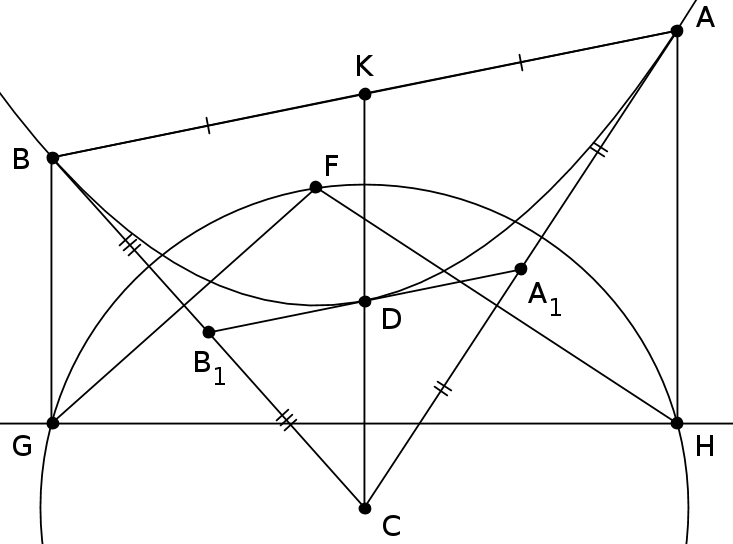
\includegraphics{pictures/2012-2013-3}
\end{center}

Свойство 1. $C$ --- центр описанной окружности треугольника $FGH$. Согласно оптическому свойству параболы: $AC$ --- биссектриса $\angle FAH$. А согласно определению $AF = AH$. Значит $AC$ --- серединный перпендикуляр к $FH$. Аналогично $BC$ --- серединный перпендикуляр к $FG$. 

Свойство 2. прямая $KC$ параллельна оси симметрии параболы и равноудалена от $AH$ и $BG$. Из свойства 1, $KC$ --- серединный перпендикуляр к $GH$. А точка $K$ равноудалена от прямых $AH$ и $BG$, поэтому $KC$ параллельна оси симметрии.

Обозначим $D$ --- точку пересечения $KC$ и параболы, $A_1$ и $B_1$ --- пересечение касательной к параболе в точке $D$ c прямыми $CA$ и $CB$. 

Свойство 3. $A_1B_1$ --- средняя линия треугольника $ABC$. Согласно свойству 2, $A_1$ равноудалена от прямых $KC$ и $AH$, а $B_1$ равноудалена от $KC$ и $BG$. Значит, $AA_1 = A_1C$ и $BB_1 = B_1C$. 

\item (Абдикалыков А.К.) Ответ: 4, 5, 6, 7. Перепишем это равенство в виде $\displaystyle\sum\limits_{k=2}^n{\left[\sqrt[k]{n}~\right]}=n$. В левой части полученного соотношение находится сумма $n-1$ натурального числа, расположенного в порядке невозрастания, следовательно, $\left[\sqrt{n}~\right]=2$, $\left[\sqrt[3]{n}~\right]=1$. Выводим $n\in\left\{4, 5, 6, 7\right\}$; все эти значения удовлетворяют исходному равенству.


\item Ответ: 981. Подходящие числа записываются в троичной системе счисления только цифрами 0 и 1. Таким образом, запись искомого числа в троичной системе счисления совпадает с двоичной записью числа 100: $$100 = 64 + 32 + 4 = 1100100_2.$$
Ответ на задачу: $$3^6 + 3^5 + 3^2 = 729 + 243 + 9 = 981.$$

\item Умножив обе части данного равенства на $A^n$ слева, получим $a_0=0$ и исключим единичную матрицу из равенства. Умножим теперь то же равенство на $A^{n-1}$, получим $a_1=0$ и исключим уже $A$ в первой степени. Продолжая этот процесс, получим требуемое. Доказательство утверждения в обратную сторону тривиально.

\item Ответ: $\frac{4}{3} (\pi^2 - 9)$. Достаточно воспользоваться тождеством:
$$\frac{1}{1^3 + 2^3 + \hdots + k^3} = 4 \left(\frac{1}{k} - \frac{1}{k+1}\right)^2.$$

\item Никакие две из указанных 12 клеток не могут быть заняты или быть побиты одним конем.

\begin{center}
\begin{tikzpicture}[x=8,y=8]
\draw[step=1] (0,0) grid (8, 8);
\draw[fill] (0,0) rectangle (1, 1);
\draw[fill] (0,1) rectangle (1, 2);
\draw[fill] (1,1) rectangle (2, 2);

\draw[fill] (6,1) rectangle (7, 2);
\draw[fill] (6,0) rectangle (7, 1);
\draw[fill] (7,0) rectangle (8, 1);

\draw[fill] (6,6) rectangle (7, 7);
\draw[fill] (7,6) rectangle (8, 7);
\draw[fill] (7,7) rectangle (8, 8);

\draw[fill] (0,7) rectangle (1, 8);
\draw[fill] (1,7) rectangle (2, 8);
\draw[fill] (1,6) rectangle (2, 7);
\end{tikzpicture}
\end{center}

\item Воспользуемся неравенством:
$$\int\limits_{0}^{1} \left(f(x) - ax - b\right)^2\,dx \geqslant 0,$$
которое верно для любых $a, b \in \mathbb{R}$. $a$ и $b$ выбираются соответствующим образом.

\end{enumerate}


\newpage

\header{2013--2014}{20 декабря 2013}
\begin{enumerate}
\item Ответ: можно. Одно из возможных решений:

\begin{center}
\begin{tikzpicture}[x=7,y=7]
\draw[step=1] (0,0) grid (3, 3);
\draw[step=1] (4,0) grid (6, 2);
\draw[step=1] (7,0) grid (9, 1);
\draw[step=1] (0,4) grid (1, 8);

\draw[step=1] (3,4) grid (9, 8);
\draw[step=1] (5,3) grid (9, 4);
\draw[step=1] (7,2) grid (9, 3);
\end{tikzpicture}
\end{center}

\item Ответ: 0. Прибавив к первой строке все остальные, получим нулевую строку, так как по теореме Виета сумма корней равна нулю.

\item Докажем, что касательные к параболе, проведенные из любой точки на директрисе параболы, --- взаимно перпендикулярны.

$F$ --- фокус, $d$ --- директриса, $AB$ --- хорда параболы, проходящая через фокус $F$, $A_1$, $B_1$ --- проекции $A$, $B$ на $d$. 

\begin{center}
%\input{solution/pictures/2013-2014-3}
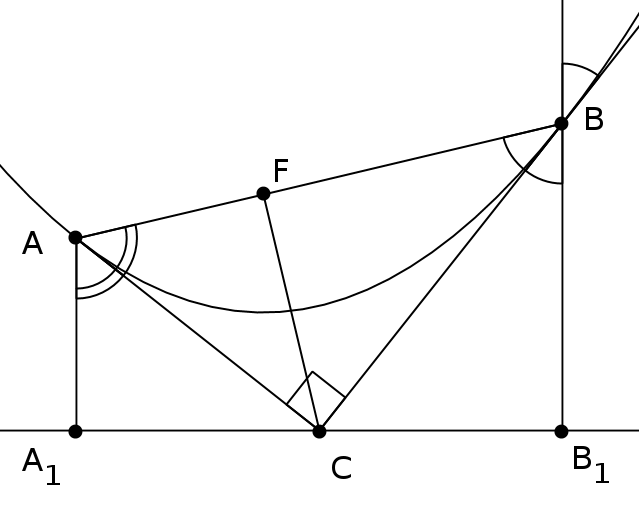
\includegraphics{pictures/2013-2014-3}
\end{center}

Свойство 1. Касательные к параболе, проведенные в концах хорды $AB$, взаимно перпендикулярны. Утверждение легко получить с учетом того, что прямые $AA_1$ и $BB_1$ параллельны, а $AC$ и $BC$ --- биссектрисы углов $\angle ABB_1$ и $\angle BAA_1$ (согласно оптическому свойству).

Свойство 2. $C$ --- точка пересечения касательных --- лежит на директрисе. В силу равенства треугольников $\Delta AA_1C$ и $\Delta AFC$, $\Delta BB_1C$ и $\Delta BFC$, получаем $\angle A_1CB_1 = \pi$.


\item Последовательно полагайте в исходном соотношении:
\begin{enumerate}
\item $a = x$, $b = 0$, $c = 0$;
\item $a = x * 0$, $b = 0$, $c = y$;
\item $a = 0$, $b = x$, $c = 0$;
\item $a = 0 * x$, $b = 0$, $c = y$.
\end{enumerate}

\item а) Количество интересных перестановок порядка $N$ вычисляется с помощью формулы включения-исключения:
$$S(N) = N!-{\frac {N!}{1!}}+{\frac {N!}{2!}}-{\frac {N!}{3!}} + \dots +(-1)^{N}{\frac {N!}{N!}}=\sum _{k=0}^{N}(-1)^{k}{\frac {N!}{k!}}
$$

б) $e^{-1}$.

\item Ответ: $k = 2$. Замена: $t = \ln{x}$. Тогда
$$\int\limits_{1}^{2} \left( 1 + k \ln{x} \right) x^{x^k + k - 1} dx = \int\limits_{0}^{\ln{2}} \left(e^{te^{kt}} \right)' dt = $$
$$=\left. e^{te^{kt}} \right|_{0}^{\ln{2}} = 2^{2^k} - 1.$$

\item a) Для любого целого $n$ куб $n$ может давать при делении на 9 только следующие остатки: 0, 1 или 8. Следовательно, числа вида $9k \pm 4$ не могут быть представлены в виде суммы трех кубов.

б) Используйте тождество:
$$6x = (x+1)^3 + (x-1)^3 + (-x)^3 + (-x)^3.$$

\item Ответ: $\frac{(n/2)!}{(n/4)!}$. Из условия следует, что для любого $k$ от 1 до $n$ верно $f(f(k)) = n + 1 - k$, то есть определить $f(f(k))$ можно однозначно. Также очевидно, что $f^4(k) = k$. Из четности $n$ понятно, что $f^2(k) \neq k$. Следовательно, $f(k) \neq k$ и $f^3(k) \neq k$. 

В качестве $f(1)$ можно выбрать любое значение из $n-2$ (кроме 1 и $n$). Сразу однозначно определяются значения $f(1)$, $f(f(1))$ и $f(f(f(1)))$. Далее для $s$ (любых из $n-4$ еще неопределенных значений) можно выбрать любое из $n-6$ допустимых значений (кроме уже определенных 4 значений, $s$ и $n+1-s$). Итог ($n = 4m$):
$$(n-2) \cdot  (n-6) \cdot  ... \cdot  6 \cdot 2 = \frac{(2m)!}{m!}.$$

\item Ответ: $2 - \frac{1}{2^n}$.

Ясно, что многочлен $x P(x) - 1$ имеет степень $n+1$. Его корнями при этом будет $n+1$ число: $2^k$ при $k$ от $0$ до $n$. Значит, этот многочлен представляется в виде 
$$x P(x) - 1 = A (x - 1) (x - 2) ... (x - 2^n).$$
Коэффициент $A$ можно найти, приравнивая свободный член: $A = (-1)^{n+1} \frac{1}{2^{1+2+...+n}}$. Свободный член $P(x)$ равен коэффициенту при $x^1$ в правой части:
$$ - \left(1 + \frac{1}{2} + ... + \frac{1}{2^n} \right).$$

\item Ответ: $\frac{k^2 + k + 2}{2}$. Выберем некоторую вершину $A$: на расстоянии 1 от неё расположено $k$ вершин (обозначим это множество вершин $B$), а на расстоянии 2 ---  $(n - 1 - k)$ вершин (обозначим это множество вершин $C$). Посчитаем количество различных четырехугольников. 

Способ первый: вершины, противоположные $A$ в соответствующем четырехугольнике, обязательно содержатся в $C$. Каждая такая вершина определяет четырехугольник однозначно. Значит, общее количество четырехугольников в графе $\frac{n(n-k-1)}{4}$.

Способ второй: соседи вершины $A$ обязательно содержатся в $B$. Каждая такая пара определяет четырехугольник однозначно. Значит, общее количество четырехугольников в графе $\frac{nk(k-1)}{8}$.

Приравниваем данные соотношения и получаем:
$$n = \frac{k^2 + k + 2}{2}.$$

\end{enumerate}

\newpage

\header{2013--2014 (дополнительный тур)}{15 марта 2014}
\begin{enumerate}

\item Операцию деления пополам можно получить следующим образом: 
$$\frac{x}{2} = \frac{1}{\frac{1}{x} + \frac{1}{x}}$$
А операцию умножения так: 
$$a b = \left( \frac{a+b}{2} \right)^2 - \left( \frac{a-b}{2} \right)^2.$$

\item Ответ: 1. По теореме Виета: $\alpha \beta \gamma = 1$, $\alpha \beta + \beta \gamma + \gamma \alpha = -1$, $\alpha + \beta + \gamma = 0$.
Используя уравнения, заменим 
$$ \frac{1-\alpha}{1+\alpha} = \frac{\alpha^3 - 2 \alpha}{\alpha^3}.$$
Осталось заметить, что:
$$\frac{1}{\alpha^2} + \frac{1}{\beta^2} + \frac{1}{\gamma^2} = (\alpha \beta + \beta \gamma + \gamma \alpha)^2 - 2 (\alpha + \beta + \gamma) = 1.$$


\item Ответ: 25. Пример:
$$
\begin{pmatrix}
4 & 1 & -1 \\
-1 & 1 & -1 \\
-1 & 1 & 4 \\
\end{pmatrix}
$$

Первый случай: если 4-ки стоят на позициях, в которых сумма индексов разной четности, то определитель равен:
$$\Delta = 4 \cdot s_1 + 4 \cdot s_2 + 4 \cdot s_3 + 4 \cdot s_4 + s_5 + s_6,$$
где $s_i = \pm 1$. Легко понять, что он не больше 18.

Второй случай: если 4-ки стоят на позициях, в которых сумма индексов одинаковой четности, то определитель равен:
$$\Delta = 4 \cdot 4 \cdot s_1 + 4 \cdot s_2 + 4 \cdot s_3 + s_4 + s_5 + s_6.$$
Ясно, что этот определитель не превосходит 27 и является нечетным. Достаточно показать, что все $s_i$ одновременно не могут быть 1.

\item Ответ: $\frac{\sqrt{3}}{3} \pm \frac{i}{2}$. После замены $t = \frac{1}{z}$ система примет вид:
\begin{equation*}
\begin{cases}
|t| = 1\\
t + t^{11} = \sqrt{3}
\end{cases}
\end{equation*}
Откуда легко получить, что $|t - \sqrt{3}| = 1$. Значит, решения могут находиться только среди точек пересечения единичных окружностей в центрами в $(0; 0)$ и $(\sqrt{3}; 0)$.

\item Ответ: $\frac{\pi}{4}$. Разобьем интеграл по области интегрирования на два и сделаем замену $x = -t$ в первом:
$$\int\limits_{-1}^{0} \frac{dx}{(e^x + 1)(x^2 + 1)} + \int\limits_{0}^{1} \frac{dx}{(e^x + 1)(x^2 + 1)} = $$
$$= \int\limits_{0}^{1} \frac{dt}{(e^{-t}+ 1)(t^2 + 1)} + \int\limits_{0}^{1} \frac{dx}{(e^x + 1)(x^2 + 1)} = $$
$$= \int\limits_{0}^{1} \frac{dx}{x^2 + 1} = \frac{\pi}{4}.$$

\item Известно, что $P$ --- центр описанной окружности треугольника $AFB$ (см. задачу 3 из олимпиады 2012--2013). Значит, $\angle FPX = \angle FBA = \angle FYP$. То есть треугольники $FYP$  и $FPX$ подобны.
\begin{center}
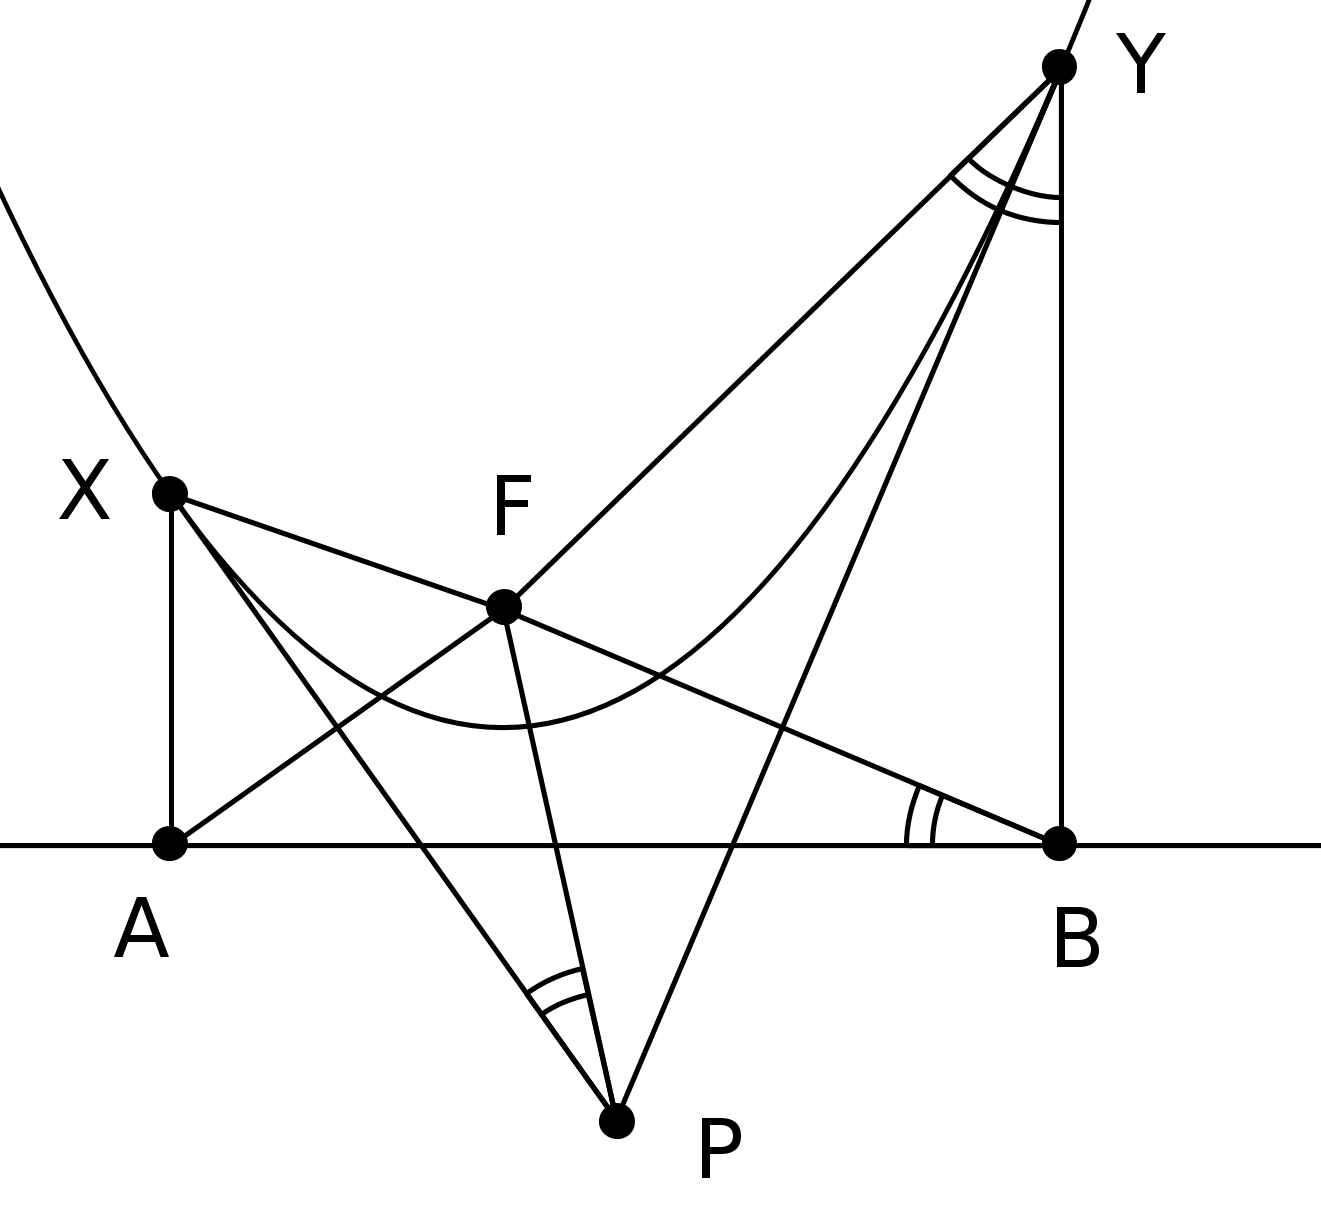
\includegraphics[width=0.5\linewidth]{pictures/2013-2014-bonus-6}
\end{center}

\item (Баев А.Ж.) Утверждение: $f^{2014}(x) = x$ имеет решение тогда и только тогда, когда $f(x) = x$ имеет решение. Легко доказывается от противного для произвольного уравнения $f^k(x) = x$ при $k>1$.

Пусть $f(x) \neq x$. Легко показать, что $f(x_v) > x_v$, где $x_v$ --- вершина параболы. Это значит, что множество значений $f(x)$ вложено в область возрастания $f(x)$. То есть $f(x) \geqslant f(x_{min}) > x_{min}$. Значит, минимальное значение $f^{k+1}(x)$ будет больше, чем минимальное значение $f^{k}(x)$.

\item (Баев А.Ж.) Композицией мы можем получить функции:
$$s(x) = \ctg (\arctg (x) ) = \frac{1}{x};$$
$$h(x) = \ctg (\arctg ( \cos ( \arctg(x) ) ) ) = \sqrt{x^2+1}.$$
Применив $k$ раз функцию $h(x)$, можно получить:
$$g_k(x) = h(h( ... h(x) ... )) = \sqrt{x^2 + k}.$$

Для всех $n \in \mathbb{N}, n > 1$ существует такое $k = n^2-1$, что $g_k(1) = n$. То есть, для любого натурального существует композиция такая, что  $R(1) = n$.

Рассмотрим 
$$g_2(s(x)) = \sqrt{\frac{1+2x^2}{x^2}}.$$
Если в качестве $x$ положить $n$ (из условия $m^2 - 2n^2 = 1$), то получим $g_2(s(n)) = \frac{m}{n}$.

\item Индукцией по $l$ доказывается, что
$$H_{2^l} = 1 + \frac{1}{2} + \frac{1}{3} + \hdots + \frac{1}{2^l} \leqslant l + 1.$$
Далее, с учетом того, что $p_i < 2^{100}$:
$$\left( \sum_{i=1}^{n} \frac{1}{p_i} \right)^k < k! \sum_{1 \leqslant i_1 \leqslant \hdots \leqslant i_n \leqslant n} \frac{1}{p_{i_1} p_{i_2} \hdots p_{i_k}} \leqslant $$
$$ \leqslant k! ( H_{2^{100k}} - 1) \leqslant (100 k) k!,$$
откуда
$$\sum_{i=1}^{n} \frac{1}{p_i} < \bigl( (100 k) \cdot k! \bigr) ^{\frac{1}{k}}.$$
Здесь $k$ --- любое натуральное. Положим $k = 4$.
\end{enumerate}


\newpage

\header{2014--2015}{10 декабря 2014}
\begin{enumerate}
\item Ответ: $f(x) = x - \frac{3}{2}$. Рассмотрим функцию 
$$g(x) = f(x) - \left(x - \frac{3}{2}\right).$$
Она непрерывна и удовлетворяет соотношению 
$$g(2x+1) = \frac{1}{3} g(x),$$ 
для любого $x \in \mathbb{R}$. После замены $t = 2x+1$:
$$g(t) = \frac{1}{3} g\left( \frac{t-1}{2} \right).$$
Отсюда $g(-1) = 0$. Далее, для каждого $y \in \mathbb{R}$ рассмотрим последовательность, заданную рекуррентным способом: 
$$\begin{cases}
y_1 = y, \\
y_{n+1} = \frac{y_n-1}{2}.
\end{cases}$$
Тогда $\lim_{n \to \infty} {y_n} = -1$ и $g(y_n) = \frac{1}{3} g(y_{n+1})$ для всех $y \in \mathbb{R}$. 
Значит,
$$g(y) = \frac{1}{3^n} g(y_{n}).$$
В силу непрерывности имеем $g(y) = 0$.  

\item Ответ: $-\frac{\pi^2}{18}$.

Во-первых:
$$
\int\limits_{0}^{1} \frac{\ln(1-u)}{u} \,du = 
\{ u = v^2 \} = 
2 \int\limits_{0}^{1} \frac{\ln(1-v^2)}{v} \,dv = $$
$$=2 \left( 
\int\limits_{0}^{1} \frac{\ln(1-v)}{v} \,dv 
+
\int\limits_{0}^{1} \frac{\ln(1+v)}{v} \,dv
\right),
$$
то есть
$$
\int\limits_{0}^{1} \frac{\ln(1-u)}{u} \,du = 
-2 \int\limits_{0}^{1} \frac{\ln(1+v)}{v} \,dv .
$$

Во-вторых:
$$
\int\limits_{0}^{1} \frac{\ln(1-u)}{u} \,du = 
\{ z = v^3 \} = 
3 \int\limits_{0}^{1} \frac{\ln(1-z^3)}{z} \,dz$$


\item Ответ: нет. Для некоторого $N \in \mathbb{N}$:
$$\sum_{n=1}^{\infty} \frac{\varepsilon_n}{n!} =
\sum_{n=1}^{N} \frac{\varepsilon_n}{n!} +
\sum_{n=N+1}^{\infty} \frac{\varepsilon_n}{n!} =
\frac{H}{N!} + r_N,$$
где $H \in \mathbb{Z}$ и 
$$|r_N| \leqslant \sum_{n=N+1}^{\infty} \frac{1}{n!} = \frac{1}{(N+1)!} \left( 1 + \frac{1}{N+2} + ... \right) < $$
$$ < \frac{3}{2} \cdot \frac{1}{(N+1)!} < \frac{1}{N!}.$$
При этом $r_N \neq 0$, так как $r_{N} = \frac{1}{(N+1)!} \varepsilon_{N+1} + r_{N+1}$ и $|r_{N+1}| < \frac{1}{(N+1)!}$.

\item (Абдикалыков А.К.) Пусть $f(\lambda) = |B-\lambda I|$ --- характеристический многочлен матрицы $B$. Заметим, что требуется доказать то, что $f(1)\ne 0$; другими словами, то, что число 1 не является собственным значением матрицы $B$. А поскольку из $AB=A+2014B$ следует $(A-2014I)(B-I)=2014I$, то матрица $B-I$ обязана быть невырожденной.

\item Ответ: при четном $n$ выиграет начинающий, а при нечетном --- его соперник. Легко заметить, что если текущее число нечетное, то игрок изменит число на четное; а если четное, то игрок всегда может уменьшить число на 1.

\item Пусть $x$ таково, что $x^3-x-1=0$. Но тогда
$$
x^5-x^4-1=(x^2-x+1)(x^3-x-1)=0.$$

\item Ответ: $\frac{\pi}{4}$. Из тождества 
$$F_{n-1}F_{n+1}=F^2_n+(-1)^n$$
можно получить соотношение $$\mathrm{arcctg}\,{F_{2n+1}}=\mathrm{arcctg}\,{F_{2n}}-\mathrm{arcctg}\,{F_{2n+2}}.$$
Искомая сумма, таким образом, будет равна $$\mathrm{arcctg}\,{F_2}=\pi/4.$$

\item Все перестановки, обратные сами себе, можно представить в виде композиции непересекающихся циклов длины 2. Число перестановок $\alpha$ порядка $n+1$ таких, что $\alpha=\alpha^{-1}$ и $\alpha_{n+1}=n+1$, очевидно, равно $a_n$; число же перестановок $\alpha$ порядка $n+1$ таких, что $\alpha=\alpha^{-1}$ и $\alpha_{n+1}=k\not=n+1$ для некоторого фиксированного $k$, равно $a_{n-1}$. Общее число инволюций порядка $n+1$ равно $a_{n+1} = a_n + na_{n-1}$.

\item (Баев А.Ж.) Ответ: 24. Пусть столбцов не меньше, чем строк. Если столбцов не менее 5, то строк менее 5. Доказательство от противного (в первой строке как минимум 3 клетки одного цвета, значит, в остальных строках обязательно найдется прямоугольник с клетками противоположного цвета). Если строк 3 или 4, то столбцов менее 7 (доказательство аналогично предыдущему). 

Так как столбцов не более 6, строк не более 4, то ответ 24. Пример:
\begin{center}
\begin{tabular}{|c|c|c|c|c|c|}
\hline
A & A & A & B & B & B \\
\hline
A & B & B & B & A & A \\
\hline
B & A & B & A & B & A \\
\hline
B & B & A & A & A & B \\
\hline
\end{tabular}
\end{center}

\item Обозначим: $KLM$ --- исходный треугольник, $A$, $B$, $C$ --- точки касания параболы и прямых $MK$, $KL$, $LM$. $A_2$, $B_2$, $C_2$ --- проекции $A$, $B$, $C$ на директрису. $F$ --- фокус параболы. $A_1$, $B_1$, $C_1$ --- середины $A_2F$, $B_2F$, $C_2F$.

\begin{center}
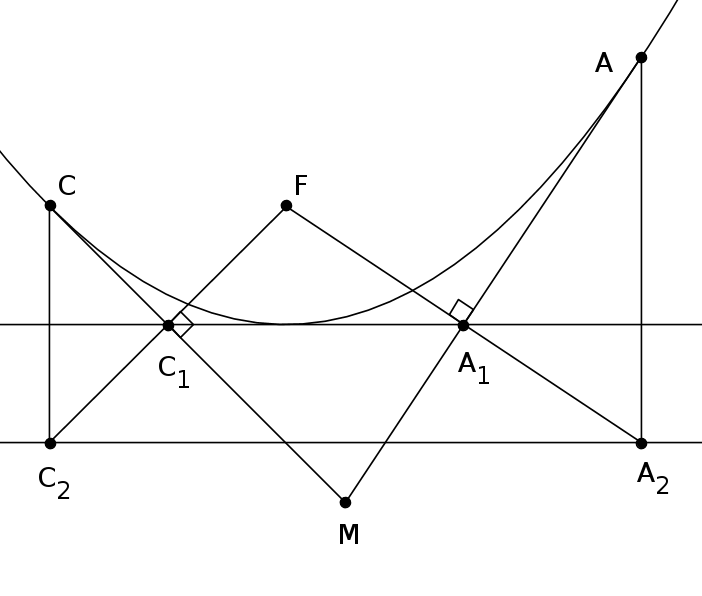
\includegraphics{pictures/2014-2015-10-1}
\end{center}

Свойство 1. Прямая, содержащая $A_1B_1C_1$, является касательной к параболе и параллельна директрисе. Данный факт легко получить из оптического свойства параболы и определения параболы (треугольник $FAA_2$ --- равнобедренный).

Свойство 2. Треугольники $FA_1K$ и $FC_1L$ подобны. Данный факт получается из вписанных четырехугольников $FKA_1B_1$ и $FB_1LC_1$.

Обозначим: $L_1$ --- основание высоты из $L$ на $KM$, $K_1$ --- основание высоты из $K$ на $LM$. $P$ и $Q$ --- точки пересечения $LL_1$ и $KK_1$ с $A_1C_1$.

\begin{center}
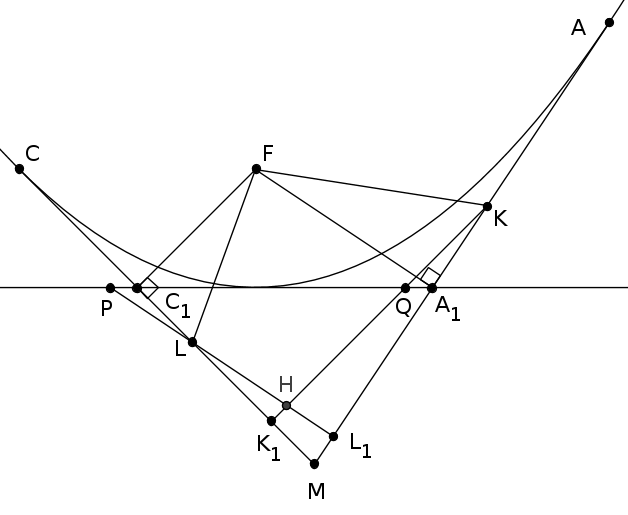
\includegraphics[width=8cm]{pictures/2014-2015-10-2}
\end{center}

Свойство 3. $A_1Q = PC_1$. По соответствующим теоремам синусов для треугольников $PC_1L$, $KA_1Q$ и $C_1FA_1$ можно получить, что 
$$ \frac{PC_1}{A_1Q} = \frac{C_1L}{A_1K} \cdot \frac{\sin Q}{\sin P} = \frac{C_1L}{A_1K} \cdot \frac{\sin C_1}{\sin A_1} = \frac{C_1L}{A_1K} \cdot \frac{A_1F}{C_1F} = 1$$
Последнее верно из свойства 2.

Свойство 3. $H$ лежит на директрисе. Для этого достаточно заметить, что треугольники $PHQ$ и $A_1FC_1$ равны. Значит, расстояние от $H$ и $F$ до прямой $A_1C_1$ одинаково.


\end{enumerate}
\newpage

\header{2015--2016}{19 декабря 2015}
\begin{enumerate}

\item (Абдикалыков А.К.) Пусть $z_n=a_nb_n-x_ny_n$. Видно, что $z_n$ можно представить в виде $z_n=\alpha n^2+\beta n+\gamma$ для некоторых постоянных $\alpha$, $\beta$, $\gamma$. Но так как $z_n$ обращается в ноль при трёх различных $n$, то $\alpha=\beta=\gamma=0$, и $z_n$ тождественно равно нулю.

\item Ответ: 12090. Положим $n$ простым: $f(n) = f(1) - f(n)$. То есть 
$$f(p) = \frac{1}{2}f(1)$$
для любого простого $p$.

Положим $n = p_1^{\alpha_1} p_2^{\alpha_2} ... p_s^{\alpha_s}$ и обозначим 
$$k(n) = \alpha_1 + \alpha_2 + ... + \alpha_s.$$
Несложно показать, что:
$$f(n) = \left( 1 - \frac{k(n)}{2} \right) f(1).$$
Имеем $2015 = 5^1 \cdot 13^1 \cdot 31^1$ и $2016 = 2^5 \cdot 3^2 \cdot 7^1$. Соответственно $k(2015) = 3$, $k(2016) = 8$.

\item Ответ: $f(x) \equiv 0$. Пусть $n \in \mathbb{Z}$. Тогда $f'(n) = f'(n+1) = 0$, откуда $f(n) = f(n+1) = 0$. Докажем от противного, что $f(x) = 0$ для всех $x \in [n, n+ 1]$. Пусть $x_0 \in (n, \,n+1)$ и $f(x_0) \neq 0$, например, $f(x_0) > 0$. Т.к. $f$ дифференцируема, то $f$ --- непрерывна на $[n, n+1]$. По теореме Вейерштрасса у нее существует максимум на $[n, n+1]$: 
$$f(x_1) = \max\limits_{[n, n+1]} f(x) > 0 \text{ и } x_1 \in (n, n+1).$$

По теореме Ферма имеем: $f'(x_1) = 0$, откуда $f(x_1) = 0$ --- противоречие.

\item Так как парабола является коническим сечением, то можно осуществить проективное преобразование с точкой в вершине соответствующего конуса, переводящее параболу в окружность. Дан вписанный четырехугольник $B_1B_2B_3B_4$. Касательные в $B_1$ и $B_2$ пересекаются в точке $K$, касательные в $B_3$ и $B_4$ в точке $L$. Осталось доказать, что $KL$, $B_1B_3$ и $B_2B_4$ пересекаются в одной точке.

\begin{center}
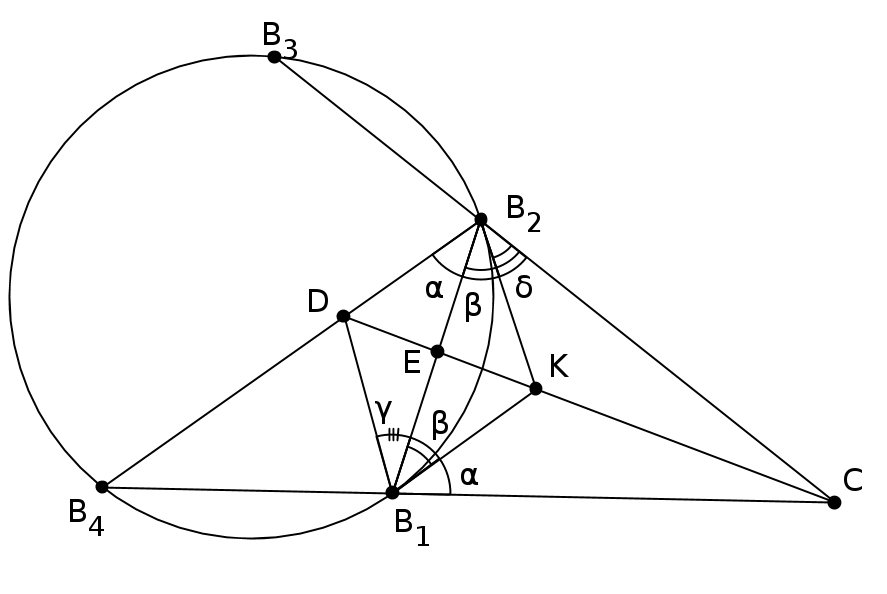
\includegraphics[width=0.8\linewidth]{pictures/2015-2016-4}
\end{center}

Пусть $C$ --- точка пересечения $B_1B_4$ и $B_2B_3$. $E$ и $K$ --- точки пересечения $CK$ с $B_1B_2$ и $B_4B_2$. Обозначим $\angle DB_2E = \angle CB_1K = \alpha$, $\angle EB_2K = \angle EB_1K = \beta$, $\angle KB_2C = \delta$ и $\angle DB_1B_2 = \gamma$. Выпишем двойные отношения (по теоремам синусов) от вершин $B_1$ и $B_2$ соответственно:
$$ \frac{\sin{\alpha}}{\sin{\beta}}: \frac{\sin(\alpha+\beta+\gamma)}{\sin{\gamma}} = \frac{CK}{KE} : \frac{CD}{DE}$$

$$\frac{\sin{\delta}}{\sin{\beta}}: \frac{\sin(\alpha+\beta+\delta)}{\sin{\alpha}} = 
\frac{CK}{KE} : \frac{CD}{DE}$$

Откуда получаем $\delta = \gamma$, то есть $D$ --- точка пересечения диагоналей. Аналогично доказывается, что $D$ лежит на $CL$. Итог: $KL$ проходит через точку пересечения диагоналей.

\item (Абдикалыков А.К.) Ответ: $-3\pi$. 

Очевидно, что $x=-3\pi$ является одним из решений. Введём функцию $f(x)=2x+\sin x$. Тогда данное уравнение можно переписать в виде $f(f(x))=-12\pi$. Поскольку функция $f(x)$ (а значит, и функция $f(f(x))$ вместе с ней) является возрастающей, то это уравнение не может иметь больше одного корня.

\item Каждому числу $a_j$ сопоставим ребро, соединяющее вершины графа с номерами $j$ и $a_j$. Полученный мультиграф имеет $n$ вершин и $n$ рёбер, и, следовательно, обязан содержать цикл. Номера вершин, входящих в любой из циклов, формируют требуемое подмножество $P$.

\item (Абдикалыков А.К.) Ответ: $(1)$ --- матрица порядка 1. Если порядок матрицы $n>1$, то из $\mathrm{rg}\,A=1$ следует вырожденность матрицы $A$, что, в свою очередь влечёт присутствие собственного значения 0. Так как след равен сумме всех собственных значений, то $\mathrm{tr}\,A=0$ --- противоречие. Удовлетворять всем условиям задачи может только матрица первого порядка, единственный элемент которой равен 1.

\end{enumerate}
\newpage

\header{2016--2017}{10 декабря 2016}
\begin{enumerate}
\item Пусть $I$ --- искомый интеграл. Сделав замену $t=2\pi-x$, получим $I=-I$; следовательно, $I=0$.

\item Так как $P(1) = 2$ и $P(2) = 1$, то многочлен $P(x)$ можно представить в виде $P(x)=(x-1)(x-2)Q(x)+3-x$ для некоторого многочлена $Q(x)$. Осталось подобрать многочлен $Q(x)$ так, чтобы для любого рационального $x$ (кроме, быть может, 1 и 2) $Q(x)$ было иррациональным. Например, подойдёт $Q(x)=\sqrt 2$. Нетрудно показать, что полученный многочлен $P(x)=\sqrt 2(x-1)(x-2)+3-x$ удовлетворяет всем указанным требованиям.

\item Заметим, что $f(x) > 0$, для всех $x \in \mathbb{R}$ и $f(-x) = f(x)$, т.е. $f(x)$ --- четная. Следовательно,
$$f(x) = \sqrt{f(x) f(-x)} = \sqrt{\prod_{i=1}^{n}(a_i^x + a_i^{-x} + 2)},$$  
при этом все множители в произведении положительны и нестрого возрастают при $x >0$.

\item Обозначим вершины $A_1$, $A_2$, $A_3$, $A_4$, а косинус двугранного угла при ребре $A_iA_j$ через $c_{ij}$. Суммарная площадь проекций трёх граней на четвёртую равна площади этой грани:
$$c_{ij} + c_{jk} + c_{ki} = 1,$$
для всех 4 возможных троек $(i, j, k)$. Решая систему из 4 уравнений с 6 неизвестными получим: $c_{12} = c_{34}$, $c_{13} = c_{24}$ и $c_{23} = c_{14}$. Также известно, что высоты тетраэдра на все 4 грани равны (например, из $A_3$ и $A_4$). Значит, равны высоты в гранях (например, из $A_3$ на $A_1A_2$ и из $A_1$ на $A_3A_4$). Это приводит к тому, что противоположные ребра равны.


\item Введём функцию
$$
f(x)=c_0x + \frac{c_1}{2}x^2 + \frac{c_2}{3}x^3 + \hdots + \frac{c_n}{n + 1}x^{n+1}.
$$
Очевидно, $f(0)=0$; из условия следует $f(1)=0$. Тогда по теореме Ролля найдётся хотя бы одно такое число $\xi\in[0,1]$, что $f'(\xi)=0$, а данное уравнение как раз можно переписать в виде $f'(x)=0$. 

\item Пусть $c \in D$ и $v \in A$. Тогда $cv \in D$ и $vc \in D$. От противного. Пусть $ cvw = 1$ для некоторого $w \in A$. Тогда $c = c^2 v w = 0$.

Пусть $a \in D$ и $x \not \in D$. Тогда $axax = 0$, откуда $a x a = 0 \cdot x^{-1} = 0$.

Пусть $c, d \in D$. Тогда $(c + d)^4 = (cd + dc)^2 = 0$. Следовательно, $c + d \in D$, откуда $cd = -dc$.

Если $a \in D$ и $x \in D$, то $axa = a \cdot (-a x) = - a^2 x = 0$.

\item (Баев А.Ж.) 
\begin{enumerate}
\item При $n$ от 3 до 8, вторая строка является полусуммой первой и третьей, следовательно, определитель 0.
\item При $n \geqslant 11$ первая и одиннадцатая строка совпадают.
\item Вычтем из $i$-й строки $(i-1)$-ю для всех $i$ с $n$ строки до $2$. Далее еще раз вычтем из $i$-й строки $(i-1)$-ю для всех $i$ с $n$ строки до $3$. Получится матрица с блоком размера $7 \times 7$, где на побочной диагонали стоят числа $-10$, а остальные элементы нули.
\end{enumerate}

\item В полученном двойном ряде можно поменять местами знаки суммирования:
$$
\sum\limits_{i=1}^{\infty}{\frac{H_i}{10^i}}=
\sum\limits_{i=1}^{\infty}{\left(\frac{1}{10^i}\cdot\sum\limits_{j=1}^{i}{\frac{1}{j}}\right)}=$$
$$=\sum\limits_{j=1}^{\infty}{\left(\frac{1}{j}\cdot\sum\limits_{i=j}^{\infty}{\frac{1}{10^i}}\right)}=
\frac{1}{9}\sum\limits_{j=1}^{\infty}{\frac{1}{j\cdot 10^{j-1}}}.
$$
Искомая сумма равна $\displaystyle\frac{10}{9}S\left(\frac{1}{10}\right)$, где $S(x)=\displaystyle\sum\limits_{n=1}^{\infty}{\frac{x^n}{n}}$. Из равномерной сходимости на множестве $[0, 1/2]$ функционального ряда $S(x)$ и ряда, полученного из него почленным дифференцированием, следует
$$
S'(x)=\sum\limits_{n=1}^{\infty}{x^{n-1}}=\frac{1}{1-x}.
$$
Так как $S(0)=0$, то $S(x)=-\ln(1-x)$. Таким образом,
$$
\frac{H_1}{10}+\frac{H_2}{100}+\frac{H_3}{1000}+ \hdots=\frac{10}{9}\ln{\frac{10}{9}}.$$
\end{enumerate}
\newpage

\header{2017--2018}{9 декабря 2017}
\begin{enumerate}
\item Пример
$$
\begin{pmatrix}
1 & 0  & 0 \\
0 &  0 & 1 \\
0 & -1 & 0 \\
\end{pmatrix}
$$

\item Пример
$$
x_n = 
\begin{cases}
1, & n \text{ --- простое},\\
0, & n \text{ --- непростое}.\\ 
\end{cases}
$$

\item Обозначим интеграл
$$
I = \int\limits_{-1}^{1} \frac{x^{2k} + 2017}{2018^x + 1} \;dx ,
$$
и сделаем замену $t = -x$.
$$
I = \int\limits_{-1}^{1} \frac{t^{2k} + 2017}{2018^t + 1} \cdot 2018^t \;dt ,
$$
После сложения данных интегралов 
$$2I = \int\limits_{-1}^{1} (x^{2k} + 2017) \;dx = \frac{2}{2k+1} + 2 \cdot 2017.$$

\item Заметим, что для функции $g(x) = 3 - \frac{9}{x}$ верно, что $g(g(g(x))) = x$. Откуда получаем систему из трех неизвестных:
$$
\begin{cases}
f(x) + f\left(3 - \frac{9}{x}\right) = x - \frac{9}{x} \\
f\left(3 - \frac{9}{x}\right) + f\left(-\frac{9}{x - 3}\right) = 3 - \frac{9}{x} - \frac{9}{3 - \frac{9}{x}} \\
f\left(-\frac{9}{x - 3}\right) + f\left(x\right) = -\frac{9}{x - 3} - \frac{9}{-\frac{9}{x - 3}}
\end{cases}
$$
для всех $x \neq 0$, $x \neq 3$. Откуда находим решение $f(x) = x - \frac32$ для всех $x \neq 0$, $x \neq 3$. С учетом непрерывности, получаем, что функция доопределяется на всех числовой прямой в таком же виде.

\item Достаточно использовать 2 факта: 

1) все лучи исходящие из фокуса параболы после отражения идут параллельно оси симметрии параболы; 

2) биссектрисы внутренних односторонних углов при параллельных прямых перпендикулярны.

\item Все нечетные $n$ подходят. Для этого достаточно вспомнить, что биномиальные коффициенты обладают свойством симметрии $C_{n}^k = C_{n}^{n-k}$. В случае четного $n$, согласно постулату Бертрана среди чисел от $n/2$ до $n$ существует простое. Причем степень данного простого числа будет нечетна, чего не может быть.

\item Замена $b_n = \pi - a_n$ дает последовательность: 
$$
\begin{cases}
b_0 = \pi - 1,\\
b_{n+1} = b_n - \sin{b_n}.\\
\end{cases}. 
$$
Правая часть $b_n - \sin{b_n}$ положительна и ограничена на $(0; \pi - 1)$. Несложно показать, что последовательность будет убывающей. Следовательно, она сходится. Предел легко найти из предельного перехода: $b = \pi n$. Так как предел должен лежать в $[0; \pi - 1]$, то это 0. Ответ: $\pi$.

\item Заметим, что $f(n, k) + f(k, n) = 2^{n + k + 1}$. Это можно доказать по индукции. Ответ: $f(n, n) = 4^n$.
\end{enumerate}

\newpage

\header{2017--2018 (дополнительный тур)}{13 марта 2018}
\begin{enumerate}
\item Последовательно для $i$ от $n$ до $2$ из $i$-й строки вычитаем $(i-1)$-ю:
$$
\det
\begin{pmatrix}
C_{0}^0 & C_{1}^1 & C_{2}^2 & \dots & C_{n-1}^{n-1} \\
0 & C_{1}^0 & C_{2}^1 & \dots & C_{n-1}^{n-2} \\
\dots & \dots & \dots & \dots & \dots \\
0 & C_{n-1}^0 & C_{n}^2 & \dots & C_{2n-3}^{n-2} \\
\end{pmatrix}
= ... = 1
$$

\item Идея.
$$
\frac{3n^2-1}{(n^3 - n)^2} = 
\frac{6n^2-2}{2 n^2 (n-1)^2 (n+1)^2} = 
$$
$$
=\frac{(n^2 + n)^2 + (n^2 - n)^2 - 2(n^2 - 1)^2 }{n^2 (n-1)^2 (n+1)^2}
=
$$
$$
=\frac{1}{2(n-1)^2} - \frac{1}{n^2}+\frac{1}{2(n+1)^2}
$$
Все слагаемые $\frac{1}{n^2}$, начиная с $n = 4$ встречаются в трех подряд идущих начальных слагаемых и в сумме сокращаются. Остаются лишь два слагаемых при $n = 2$ и одно при $n = 3$ общей суммой: $\frac{1}{2} - \frac{1}{4} + \frac{1}{8} = \frac{3}{8}$

\item $f(x) = 2 - f(x^2) = f(x^4)$. Так как функция четная, рассмотрим только положительные $x$.

Во--первых, $f(x^{4n}) = f(x)$. Пусть $0 \leqslant x < 1$. В силу непрерывности:
$$f(x) = \lim_{n \to \infty} f(x^{4n}) = f(0).$$

Во--вторых, $f(x^{\frac{1}{4n}}) = f(x)$. Пусть $x > 1$. В силу непрерывности:
$$f(x) = \lim_{n \to \infty} f(x^{\frac{1}{4n}}) = f(1).$$

В силу непрерывности и $f(1 - \varepsilon) = f(0)$, получаем, что $f(1) = f(0)$. Значит, $f(x) = const$. Из условия получаем, что $f(x) = 1$.

\item Пусть некоторый угол $n$-угольника содержит несколько углов $m$-угольников. Угол правильного $m$-угольника равен $180 \frac{m-2}{m}$. Если $m \geqslant 4$, то угол будет не менее $90^{\circ}$. Значит, $m = 3$, $n = 6$.

Пусть углы $n$-угольника и $m$-угольников равны: $n = m$. Так как сами многоугольники не совпадают, значит, есть точка на границе $n$-угольника в которой сходятся все несколько правильных $m$-угольников. То есть $180^{\circ}$ делится на $180^{\circ} \frac{n-2}{n}$, что равносильно условию $n$ делится на $n-2$, или $2$ делится на $n-2$. Получаем: $n = 4$ или $n = 3$.

Ответ: $(n, m) \in \{ (6; 3), (3; 3), (4, 4) \}$.


\item Рассмотрим функцию $g(x) = f(x) - x$:
$g(x)$ выпукла вниз, $g'(c) = 0$, $g(c) < 0$. Из выпуклости следует, что существует такая точка $a < c$, что $g(a) = g(b) = 0$. Существуют точки $a < c < b$ такие, что $f(a) = a$, $f(b) = b$.

Графики функций $f(x)$ и $f^{-1}(x)$ в квадрате $[a; b] \times [a; b]$ симметричны относительно прямой $y = x$. То есть область, ограниченная кривыми $y = x$ и $y = f(x)$, симметрична области, ограниченной кривыми $y = x$ и $y = f^{-1}(x)$:
$$
\int_{a}^{b} (f(x) + f^{-1}(x)) dx =
$$
$$= - \int_{a}^{b} (x - f(x)) dx + \int_{a}^{b} (f^{-1}(x) - x) dx + 2 \int_{a}^{b} x dx = b^2 - a^2
$$

\end{enumerate}
\newpage
%%%%%%%%%%%%%%%%%%%%

\header{Республиканская олимпиада по математике 2016}{01 апреля 2016}
\begin{enumerate}

\item (Васильев А.Н.)

Заметим, что справедливо разложение $$x^2-y^2+2x+2y = (x+y)(x-y+2).$$ Поэтому натуральное число представимо в этом виде тогда, и только тогда, когда раскладывается на произведение двух множителей одной четности. Ясно, что это все числа, которые дают остаток отличный от 2 при делении на 4.

Пример для нечетного $n$: $x = \frac{n-1}{2}$, $y = \frac{3-n}{2}$.

Пример для $n$, кратного 4: $x = y = \frac{n}{4}$.
 
\item (Васильев А.Н.) 

а) Легко понять, что функция кусочно--постоянная. Причем количество промежутков постоянства конечно и равно 10. Значит, функция интегрируема по Риману. 
\\
б) Найдем промежуток, на котором первая цифра числа $2^x$ равна $k$:
$$1 + \frac{k}{10} \le 2^x < 1 + \frac{k+1}{10},$$
$$\log_2 \left( 1 + \frac{k}{10} \right) \le x < \log_2 \left( 1 + \frac{k+1}{10} \right).$$

Тогда наш интеграл можно записать в виде суммы:
\begin{multline*}
\int\limits_{0}^{1} \alpha(x) dx = \\
= \sum_{k=0}^{9} k \left( \log_2 \left( 1 + \frac{k+1}{10} \right) - \log_2 \left( 1 + \frac{k}{10} \right) \right) = \\
= \sum_{k=0}^{9} k \left( \log_2 (k+11) - \log_2 (k+10) \right) = \\
= \sum_{k=0}^{9} k \log_2 (k+11) -  \sum_{k=0}^{8} (k + 1) \log_2 (k + 11) = \\
= 9 \log_2 20 - \sum_{k=0}^{8} \log_2 (k + 11) = \log_2 \frac{20^9}{11 \cdot 12 \cdot \ldots \cdot 19}
\end{multline*}

Требуется доказать, что
$$2^7 < \left( \frac{20^9}{11 \cdot 12 \cdot \dots \cdot 19} \right)^2 < 2^9.$$

Докажем левую часть неравенства. Заметим, что по неравенству Коши 
$$(10+k) * (20-k) < \left( \frac{10+k+20-k}{2} \right)^2 = 15^2.$$
Отсюда получается оценка слева:
$$\left( \frac{20^9}{11 \cdot 12 \cdot \ldots \cdot 19} \right)^2 > \left( \frac{20^9}{15^9} \right)^2 = \frac{2^{36}}{3^{18}}.$$

Остается доказать, что $2^{29} > 3^{18}$. Заметим, что $2^8>3^5$ и $2^5>3^3$. Перемножив три раза первое неравенство и один раз второе, получим требуемое.

Докажем правую часть неравенства. Заметим, что верно следующее неравенство:
$$(10+k) (20-k) = 200 + k (10 - k) > 200.$$

Значит, оценку справа можно получить так:
$$\left( \frac{20^9}{11 \cdot 12 \cdot \ldots \cdot 19} \right)^2 < \left( \frac{400^4 \cdot 20}{200^4 \cdot 15} \right)^2 = 2^8 \left( \frac{4}{3} \right)^2 < 2^9.$$


\item (Фольклор) Первое решение (<<наивное>>). Можно доказать более общее утверждение:

\textit{В любом конечном поле $F \ne Z_2$ сумма всех элементов равна нулю.}

Пусть $F$ --- конечное поле и $a_1$, $a_2$, ..., $a_n$ --- все его элементы. Если $F \ne Z_2$, то существует элемент $a$, отличный от нуля и единицы. Тогда $a a_1$, $a a_2$, ..., $a a_n$ попарно различны, следовательно
$$F = \{ a_1, ..., a_n \} = \{ a a_1, ..., a a_n \} .$$
Отсюда $S = \sum_{i=1}^{n} a_i = \sum_{i=1}^n a a_i = a S$, откуда следует, что $S = 0$.

Второе решение(существенно использующее структуру конечного поля). Утверждение из предыдущего решения можно доказать и по-другому. Ненулевые элементы поля образуют группу по умножению, а порядок элемента группы делит порядок группы (по теореме  Лагранжа). Следовательно, любой элемент поля $F$ является корнем многочлена $x^n - x = 0$, где $n$ --- количество элементов поля. С другой стороны, по другой теореме Лагранжа, у этого многочлена не более $n$ корней. Иными словами, указанный многочлен имеет своими корнями все элементы поля. Применяя теорему Виета, получаем требуемое. 

Третье решение (еще одно). У каждого ненулевого элемента $x$ есть обратный $x^{-1}$, причем $x \ne x^{-1}$ при $x \ne \pm 1$. Следовательно, все ненулевые элементы, кроме $\pm 1$, разбиваются на пары с произведением 1. Поэтому произведение всех элементов поля равно $-1$. Из условия задачи следует, что $-1 \ne 1$. Следовательно, характеристика поля отлична от 2. Тогда любой ненулевой элемент отличается от своего противоположного, то есть все ненулевые элементы разбиваются на пары с нулевой суммой. Что означает, что сумма всех ненулевых элементов поля равна нулю. Добавление нуля сумму не изменяет. Утверждение доказано.    

\item  (Баев А.Ж.) 

Факт 1 (оптическое свойство эллипса): луч, направленный из одного фокуса после отражения от внутренней стороны эллипса проходит через другой фокус. То есть $\angle(F_1M, SM) = \angle(SM, F_2M)$, где $\angle(l_1, l_2)$ обозначает ориентированный угол между прямыми. Как следствие, получаем, что $\angle F_1MS + \angle F_2MS = \pi$. По условию, $\angle F_2MS = \angle DMS$. Откуда получаем, что $F_1$, $M$, $D$ лежат на одной прямой. Аналогично, $F_2$, $N$, $E$ лежат на одной прямой.

Факт 2 (определение эллипса). Сумма расстояний от фокусов до точек на эллипсе постоянна. Как следствие $F_1M + MF_2 = F_1N + NF_2$. Так как треугольники $F_2MS$ и $DMS$ симметричны относительно прямой $MS$, то и треугольники $F_1MF_2$ и $AMD$ тоже симметричны и, соответственно, равны. Аналогично, симметричны и равны треугольники $F_1NF_2$ и $BNE$.

\begin{center}
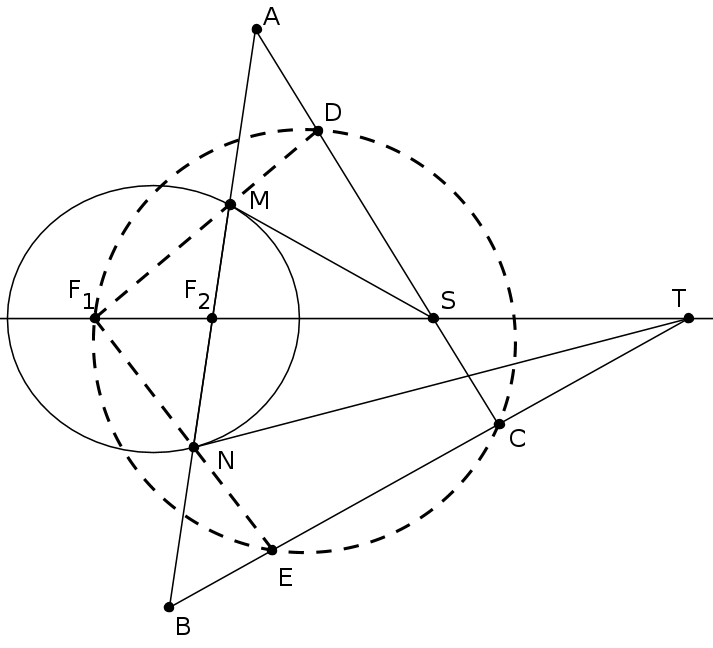
\includegraphics[width=8cm]{pictures/2016-republic}
\end{center}

а) 
$$AF_2 = AM + MF_2 = F_1M + MF_2 =$$
$$= F_1N + NF_2 = BN + NF_2 = BF_2.$$ 
Значит, $CF_2$ --- медиана треугольника $ABC$.

б) Четырехугольник $F_1DCE$ вписан в окружность, так как $\angle F_1DC + \angle F_1EC = \angle MF_2S + \angle NF_2S = \pi$. Так как в этом четырехугольнике две смежные стороны равны ($F_1D = F_1E$), то $CF_1$ --- биссектриса треугольника $ABC$.

\item (Клячко А.А.)

1) Рассмотрим случай четного $n$. Тогда каждый из игроков полностью контролирует $\frac{n}{2}$ столбцов (при этом не имеет значения, кто делает первый ход). Ясно, что Максималист может сделать свои столбцы линейно независимыми и обеспечить ранг матрицы минимум $\frac{n}{2}$. Также ясно, что Минималист может сделать все свои столбцы нулевыми, ограничив ранг матрицы $\frac{n}{2}$.

Ответ для четного $n$: $\frac{n}{2}$.

2) Пусть $n$ нечетно. Тогда, если мы раскрасим клетки таблицы в черный и белый цвета в шахматном порядке, каждый из игроков будет контролировать клетки одного цвета. 

а) Пусть Максималист делает первый ход. Тогда он сможет сделать ранг матрицы максимальным, то есть равным $n$. Опишем его стратегию. Она состоит в том, что, заполняя очередную диагональную клетку, он следит за тем, чтобы соответствующий главный (угловой) минор был отличен от нуля. Это всегда можно обеспечить, поскольку этот минор разлагается по своей последней строке, а алгебраическое дополнение последнего элемента не равно нулю. 
Ответ для нечетного $n$, когда Максималист делает первый ход: $n$. 

б) Пусть Минималист делает первый ход. Тогда он сможет обеспечить равенство нулю определителя всей матрицы: заполняя очередную диагональную клетку (кроме последней), он следит за тем, чтобы соответствующий угловой минор был отличен от нуля, а в конце обнуляет определитель всей матрицы. Значит, он сможет гарантировать ранг меньше $n$. С другой стороны, Максималист сможет обеспечить, чтобы минор, полученный вычеркиванием последней строки и первого столбца, был отличен от нуля (аналогично пункту 2 а)). Тем самым, ранг матрицы будет равен по крайней мере $n-1$. 

Ответ для нечетного $n$, когда Минималист делает первый ход: $n-1$. 
 
\item (Баев А.Ж.)

1 шаг. Подставим в соотношение $x = \frac{t}{t-1}$, где $t > 1$. Получим
$$f'\left(\frac{t}{t-1}\right) = f(t) + f\left( \frac{t}{t-1} \right) .$$

Получим свойство:
$$f' \left(\frac{t}{t-1} \right) = f'(t).$$

2 шаг. Продифференцируем исходное соотношение по $x$.
$$ f''(x) = - \frac{1}{(x-1)^2} f' \left( \frac{x}{x-1} \right) + f'(x) .$$

После замены из свойства, получаем:
$$ \frac{f''(x)}{f'(x)} = 1 - \frac{1}{(x-1)^2} .$$

Уравнение интегрируется по частям:
$$ f'(x) = C e^{x + \frac{1}{x-1}}.$$

Добавим условие на бесконечности и найдем $C = 1$:
$$ f'(x) = 2 e^{x + \frac{1}{x-1}}.$$

3 шаг. Заметим, что если в исходное дифференциальное уравнение мы подставим $x = 2$, то получим $f(2) = \frac{1}{2} f'(2)$. Значит:
$$ f(2) = e^3.$$

Осталось доказать, что $e^3 < 20.16$. Заметим, что для проверки этого неравенства грубых оценок типа $e<3$ или $e<2.8$ недостаточно, требуется более точная: $e<2.72$.

\end{enumerate}
\newpage

\header{Республиканская олимпиада по МКМ 2016}{01 апреля 2016}
\begin{enumerate}

\item (Абдикалыков А.К.)

Максимальный балл давался за алгоритм с асимптотической сложностью $O(1)$ (явную формулу), промежуточные баллы --- за сложность $O(n)$ и $O(n^2)$.
\begin{multline*}
\sum\limits_{j=1}^{n^2}{[\sqrt j\,]}=
\sum\limits_{k=1}^{n}{\left(k\cdot\sum\limits_{\substack{[\sqrt j\,]=k \\ 1 \leqslant j \leqslant n^2}}{1}\right)}=
\sum\limits_{k=1}^{n-1}{\left(k\cdot\sum\limits_{\substack{[\sqrt j\,]=k \\ 1 \leqslant j \leqslant n^2}}{1}\right)}+n=\\
=\sum\limits_{k=1}^{n-1}{\left(k\cdot\sum\limits_{j=k^2}^{(k+1)^2-1}{1}\right)}+n=
\sum\limits_{k=1}^{n-1}{k(2k+1)}+n=\\
=\sum\limits_{k=1}^{n-1}{(2k^2+k)}+n=
2\cdot\frac{(n-1)n(2n-1)}{6}+\frac{(n-1)n}{2}+n=\\
=\frac{(n-1)n(4n+1)}{6}+n=
\frac{n(4n^2-3n+5)}{6}
\end{multline*}
    
\item (Абдикалыков А.К.)

а) Две полупараболы из условия задачи --- это графики функций $y=x^2$ и $y=-\sqrt{x}$ при $x\geqslant 0$. Поэтому искомая функция
$$
S(L)=\int\limits_{0}^{f^{-1}(L)}{f(x)~dx},
$$
где $f(x)=x^2+\sqrt{x}$. (В силу монотонности функции $f(x)$ корректно вводить $f^{-1}(L)$.) Так как, кроме прочего, подынтегральная функция в определении $S(L)$ положительная, то и сама функция $S(L)$ --- возрастающая. Поскольку $S(2)=1$ (это можно показать разными способами: как графически, составив квадрат, например, так и аналитически, посчитав явно интеграл), то $S(L)>1$ при $L>2$.\\
б) Найдём сначала $x_0=f^{-1}(L)$ с помощью бинарного поиска, затем вычислим
$$
S(L)=\left.\left(\frac{1}{3}x^3+\frac{2}{3}x^{\frac{3}{2}}\right)\right|_{x=0}^{x_0}=
\frac{x_0^3+2x_0^{\frac{3}{2}}}{3}=$$
$$=\frac{x_0(2x_0^2+2\sqrt{x_0}-x_0^2)}{3}=
\frac{x_0(2L-x_0^2)}{3}.
$$

\item (Баев А.Ж.)

Продифференцируем по $x$ и $y$:
$$f'(x - y) + f'(x + y) = 2 x f''(x^2 + y^2),$$
$$ - f'(x - y) + f'(x + y) = 2 y f''(x^2 + y^2).$$

Пусть $x \ne 0$, $y \ne 0$. Приравняем $f''(x^2 + y^2)$:
$$(y + x) f'(x - y) = (x - y) f'(x + y).$$

Пусть $|x| \ne |y|$.
$$\frac{f'(x + y)}{x + y} = \frac{f'(x - y)}{x - y}.$$

Зафиксируем величину $x - y = A$, отличную от нуля. Тогда выражение справа не зависит от $y$ и равно некоторой константе $2C$.
$$\frac{f'(2y + A)}{2y + A} = \frac{f'(A)}{A} = 2 C.$$

Заметим, что $t = 2y + A$ может принимать любые ненулевые значения. Значит, при $t \ne 0$:
$$f'(t) = 2Ct.$$
$$f(t) = Ct^2 + C_1.$$

При подстановке в исходное уравнение, получим: $C_1 = 0$. При $t = 0$ доопределяется из непрерывности $f'(t)$ (по соотношению в условии). Ответ: $f(t) = C t^2$.

\item (Баев А.Ж., Абдикалыков А.К.)

Пусть конечное значение $S=\sum\limits_{j=1}^{2n-1}c_j\cdot\frac{f_{j-1}+f_j+f_{j+1}}{3}$. Тогда пункт б) эквивалентен решению нижеуказанной системы линейных уравнений, причём в целых числах. Видно, что система состоит из $(2n+1)$ уравнения относительно $(2n-1)$ неизвестной.
\begin{equation*}
\begin{pmatrix}
1 & 0 & 0 & \cdots & 0 & 0 & 0 \\
1 & 1 & 0 & \cdots & 0 & 0 & 0 \\
1 & 1 & 1 & \cdots & 0 & 0 & 0 \\
0 & 1 & 1 & \cdots & 0 & 0 & 0 \\
\cdots & \cdots & \cdots & \cdots & \cdots & \cdots & \cdots\\
0 & 0 & 0 & \cdots & 1 & 1 & 0 \\
0 & 0 & 0 & \cdots & 1 & 1 & 1\\
0 & 0 & 0 & \cdots & 0 & 1 & 1\\
0 & 0 & 0 & \cdots & 0 & 0 & 1\\
\end{pmatrix}
\begin{pmatrix}
c_1 \\
c_2 \\
c_3 \\
\cdots \\
c_{2n-3} \\
c_{2n-2} \\
c_{2n-1}
\end{pmatrix}
=
\begin{pmatrix}
1 \\
4 \\
2 \\
4 \\
\cdots \\
4 \\
2 \\
4 \\
1
\end{pmatrix}
\end{equation*}

Рассматривая только первые $(2n-1)$ уравнения, мы получим систему с нижнетреугольной матрицей и определителем, равным единице, а значит, всеми уравнениями, кроме последних двух, все неизвестные определяются однозначно, принимая при этом целые значения. Таким образом, задача сводится к нахождению таких $n$, чтобы система из этих $(2n-1)$ уравнения имела решение, совместимое с дополнительными условиями $c_{2n-2}+c_{2n-1}=4$, $c_{2n-1}=1$. Решая эту систему методом Гаусса, получаем
$$
\begin{matrix}
c_1=1, & c_2=3, & c_3=-2,\\
c_4=3, & c_5=1, & c_6=0,\\
c_7=1, & c_8=3, & c_9=-2,\\
c_{10}=3, & c_{11}=1, & c_{12}=0,\\
\end{matrix}
$$
$$
\hdots
$$
Таким образом, равенства $c_{2n-2}=3$, $c_{2n-1}=1$ выполняются только в том случае, если $$2n-1=5\pmod 6,$$ или, что то же самое, $n$ кратно 3.

Пункт а) эквивалентен решению той же системы в целых числах, но уже без первого и последнего уравнений.
\begin{equation*}
\begin{pmatrix}
1 & 1 & 0 & \cdots & 0 & 0 & 0 \\
1 & 1 & 1 & \cdots & 0 & 0 & 0 \\
0 & 1 & 1 & \cdots & 0 & 0 & 0 \\
\cdots & \cdots & \cdots & \cdots & \cdots & \cdots & \cdots\\
0 & 0 & 0 & \cdots & 1 & 1 & 0 \\
0 & 0 & 0 & \cdots & 1 & 1 & 1\\
0 & 0 & 0 & \cdots & 0 & 1 & 1
\end{pmatrix}
\begin{pmatrix}
c_1 \\
c_2 \\
c_3 \\
\cdots \\
c_{2n-3} \\
c_{2n-2} \\
c_{2n-1}
\end{pmatrix}
=
\begin{pmatrix}
4 \\
2 \\
4 \\
\cdots \\
4 \\
2 \\
4
\end{pmatrix}
\end{equation*}

Фиксируя $c_1=c$ и используя все уравнения, кроме последнего ($c_{2n-2}+c_{2n-1}=4$), находим
$$
\begin{matrix}
c_1=c, & c_2=4-c, & c_3=-2, \\
c_4=2+c, & c_5=2-c, & c_6=0,\\
c_7=c, & c_8=4-c, & c_9=-2, \\
c_{10}=2+c, & c_{11}=2-c, & c_{12}=0,
\end{matrix}
$$
$$
\hdots
$$
Значит,
$$
c_{2n-2}+c_{2n-1}=
\begin{cases}
c, & 2n-2=0\pmod 6,\\
-2-c, & 2n-2=2\pmod 6,\\
4, & 2n-2=4\pmod 6.
\end{cases}
$$
Видно, что в любом случае можно подобрать такое $c$, чтобы выполнялось равенство $$c_{2n-2}+c_{2n-1}=4,$$ из чего следует, что система совместна при любом $n$.

\item  (Абдикалыков А.К.)

а) Уменьшить двоичное число на единицу: {\bf CSLAF}.

б) Поменять все биты: {\bf CLA}.

в) Поменять только старший бит: {\bf CLRCLA}.

\item (Баев А.Ж.)

а) Пусть исходный квадрат --- это квадрат $[0, 1] \times [0, 1]$ на плоскости, а центр вырезанного квадрата расположен в точке $(x_0, y_0)$. Квадрат целиком поместится, если $(x_0; y_0) \in [a, 1 - a] \times [a, 1 - a]$. 

1 шаг. Найдем центр тяжести. Запишем функцию плотности массы пластины по оси $OX$:
$$
f(x) =
\begin{cases}
1, x < x_0 - a\\
1 - 2a, x \in [x_0 - a, x_0 + a]\\
1, x < x_0 + a\\
\end{cases}
$$

Найдем проекцию центра тяжести $m$ на ось $OX$:
$$m = \frac{\int_0^1 x f(x) dx}{\int_0^1 f(x) dx} = \frac{1 - 8 a^2 x_0}{2 (1 - 4 a^2)} .$$

2 шаг. Найдем вероятность попадания центра тяжести в вырезанную часть.
$$P = P(m \in [x_0 - a; x_0 + a]) =$$
$$= P\left( \frac{1 - 8 a^2 x_0}{2 (1 - 4 a^2)} < x_0 + a \right) - P\left( \frac{1 - 8 a^2 x_0}{2 (1 - 4 a^2)} < x_0 - a \right) =$$
$$= P\left( x_0 + a > \frac{1}{2} + 4 a^3  \right) - P\left( x_0 - a > \frac{1}{2} - 4 a^3 \right). $$
Обознаим полученную разность $P_1 - P_2.$

Вычислим $P_1$. Заметим, что $x_0 + a$ равномерно распределено на $[2a, 1]$. Поэтому важно понять, попадает ли $\frac{1}{2} + 4 a^3$ в интервал $[2a, 1]$. $\frac{1}{2} + 4 a^3 < 1$ ввиду того, что $a \in [0, \frac12]$. Проверим левую границу:

$$\frac{1}{2} + 4 a^3 > 2a$$
$$ \left(a - \frac{1}{2} \right)\left(a - \varphi \right)\left(a - \overline{\varphi}\right) > 0$$
где $\varphi= \frac{-1 + \sqrt{5}}{4}$. Значит, $\frac{1}{2} + 4 a^3$ попадает в интервал $[2a, 1]$ при $a < \varphi$.

$$P_1 = 
\begin{cases}
\frac{1 - 8 a^3}{2(1 - 2a)}, &a < \varphi\\
1, &a > \varphi.
\end{cases}
$$

Аналогично вычислим $P_2$. $x_0 - a$ равномерно распределено на $[0, 1-2a]$. Поэтому важно понять, попадает ли $\frac{1}{2} - 4 a^3$ в интервал $[0, 1-2a]$. $\frac{1}{2} - 4 a^3 > 0$ ввиду того, что $a \in [0, \frac12]$. Значит:
$$P_2 = 
\begin{cases}
 \frac{1 - 4a + 8 a^3}{2(1 - 2a)}, &a < \varphi\\
0, &a > \varphi.
\end{cases}
$$

Найдем вероятность попадания центра тяжести в вырезанную часть:
$$(P_1 - P_2)^2 =
\begin{cases}
4a^2(1+2a)^2,& a \in [0, \frac{-1 + \sqrt{5}}{4}]\\
1,& a \in \left[\frac{-1 + \sqrt{5}}{4}, \frac12 \right]\\
\end{cases}
$$

б) Промоделируем методом Монте--Карло и подсчет центра тяжести, и подсчет ответа. Генерируем $N$ подходящих квадратов. У каждого из них генерируем $M$ случайных точек. Если центр тяжести данных точек находится внутри квадрата, то засчитываем этот квадрат. Иначе --- нет. Отметим, что порядок аппроксимации данного метода $O\left( \frac{1}{ \sqrt{NM} } \right)$.

\end{enumerate} 

\newpage

\header{Республиканская олимпиада по математике 2017}{13 апреля 2017}
\begin{enumerate}

\item (Абдикалыков А.)

Пусть $S=\displaystyle\sum\limits_{n=1}^{\infty}{\frac{T_n}{2^n}}$. Тогда
$$
\sum\limits_{n=1}^{\infty}{\frac{T_{n+1}}{2^n}}=2\cdot \sum\limits_{n=1}^{\infty}{\frac{T_{n+1}}{2^{n+1}}}=2\cdot \left(S-\frac{T_1}{2^1}\right)=2S-1,
$$
$$
\sum\limits_{n=1}^{\infty}{\frac{T_{n+2}}{2^n}}=4\cdot \sum\limits_{n=1}^{\infty}{\frac{T_{n+2}}{2^{n+2}}}=4\cdot\left(S-\frac{T_1}{2^1}-\frac{T_2}{2^2}\right)=4S-3,
$$
\begin{multline*}
\sum\limits_{n=1}^{\infty}{\frac{T_{n+3}}{2^n}}=8\cdot \sum\limits_{n=1}^{\infty}{\frac{T_{n+3}}{2^{n+3}}}=\\
=8\cdot\left(S-\frac{T_1}{2^1}-\frac{T_2}{2^2}-\frac{T_3}{2^3}\right)=8S-7.
\end{multline*}

Так как по условию $T_{n+3}=T_{n+2}+T_{n+1}+T_n$, то $$8S-7=4S-3+2S-1+S,$$ откуда следует $S=3$.

\item (Абдикалыков А.)

Пусть $k$-ичная запись простого числа $p$ для некоторого $k>1$ выглядит как $\overline{a_0a_1\hdots a_{k-1}}$, где $(a_0, a_1, \hdots, a_{k-1})$ --- некоторая перестановка цифр $(0, 1, \hdots, k-1)$. Тогда
$$
p = a_0\cdot k^{k-1} + a_1\cdot k^{k-2}+\hdots+a_{k-1}\cdot k^0 \equiv
$$
$$
= a_0+a_1+\hdots+a_{k-1} \pmod {(k-1)}.
$$
Поскольку сумма всех цифр равна $k(k-1)/2$, то можно сделать вывод, что число $p$ делится на $(k-1)/2$, если $k$ нечётно и на $k-1$, если $k$ чётно. Учитывая, что $p\geqslant k^{k-1}>k-1$ --- простое число, заключаем, что $k$ должно удовлетворять совокупности соотношений
$$
\left[
\begin{matrix}
\frac{k-1}{2}=1,& k = 2l+1,\\
k-1=1, & k = 2l.\\
\end{matrix}
\right.
$$
Таким образом, $k=2$ или $k=3$, а значит, достаточно перебрать числа $10_2$, $102_3$, $120_3$, $201_3$, $210_3$. Простыми среди них являются только $2=10_2$, $11=102_3$ и $19=201_3$.

\item (Клячко А.)

а) Для любого элемента $x$ порядка 2 верно $x=x^{-1}$, поэтому
$$
(ab)^2=abab=aba^{-1}b^{-1},
$$
если $a^2=b^2=e$.

б) Аналогично, для любого элемента $x$ порядка 3 верно $x^2=x^{-1}$, поэтому
\begin{multline*}
(ab)^3=ababab=ab^4aba^4b=(ab^2)(b^2a)(ba^2)(a^2b)=\\
(ab^2)(b^2a)(ab^2)^{-1}(b^2a)^{-1},
\end{multline*}
если $a^3=b^3=e$.

\item (Баев~А.)

Обозначим через $F$ фокус параболы,  через $d$ директрису параболы. Рассмотрим произвольную касательную к параболе $l$ в произвольной точке $C$.

\begin{center}
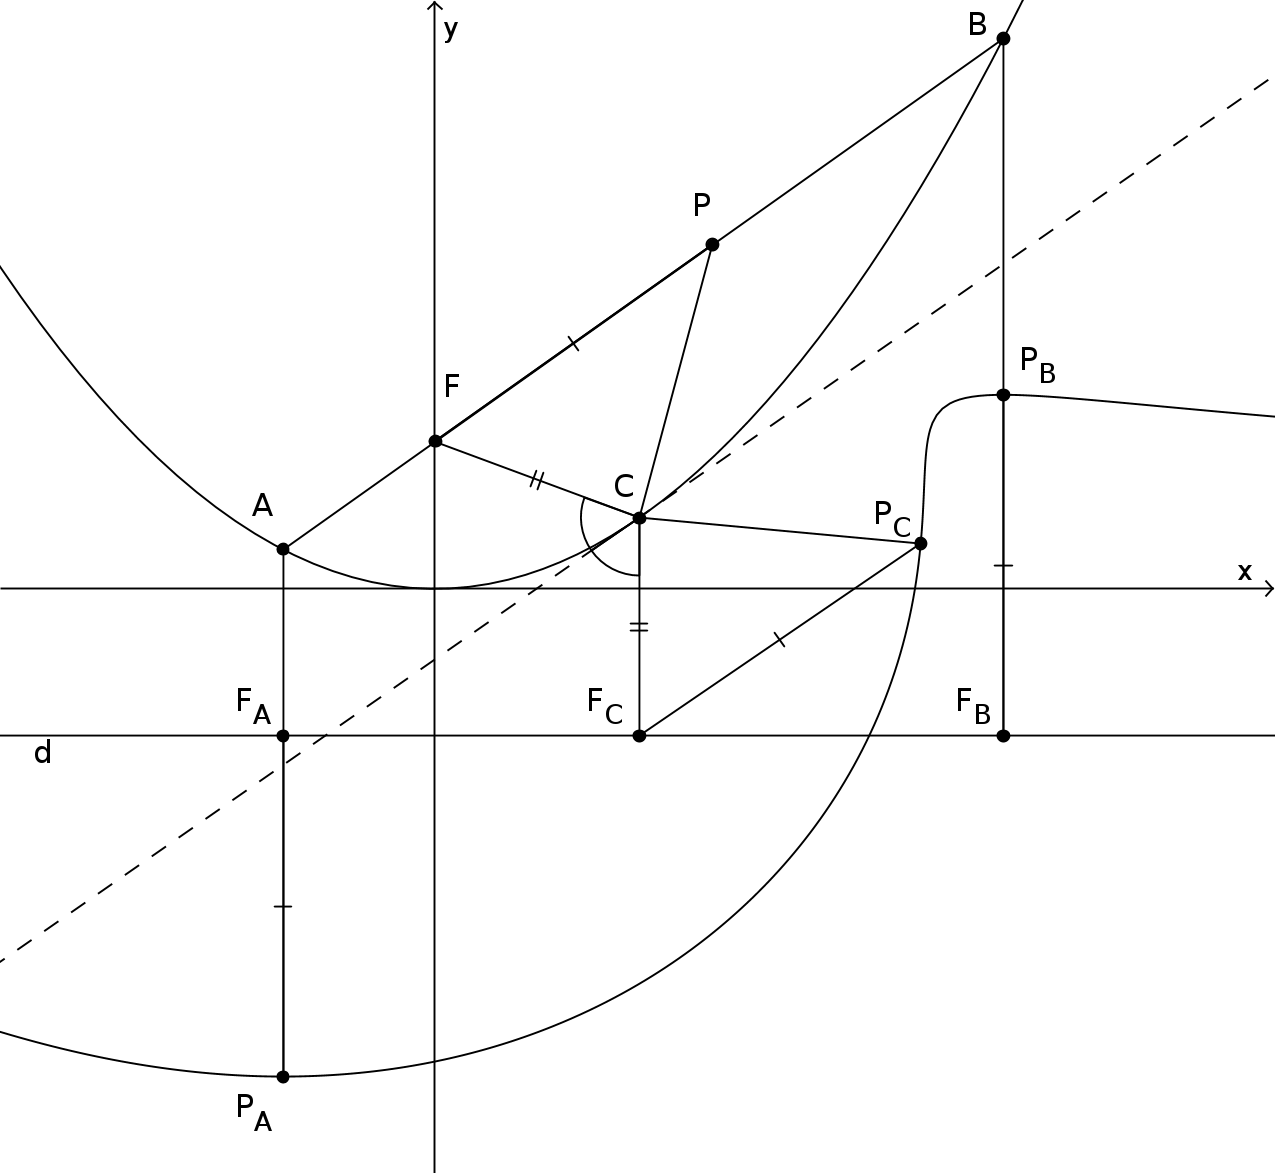
\includegraphics[scale=0.9]{pictures/2017-republic}
\end{center}

Свойство 1: точка $F_C$, симметричная $F$ относительно $l$, лежит на директрисе $d$. 

Из определения параболы: $FC = F_CC$. Из оптического свойства параболы $\angle(FC; l) = \angle(l; F_CC)$. Получаем, что $l$ --- ось симметрии для отрезков $FC$ и $F_CC$. 

Свойство 2: $$ -\frac{1}{4} - FP \leqslant y(P_C)  \leqslant -\frac{1}{4} + FP,$$
где $y(P_C)$ --- ордината точки $P_C$.

Известна директриса данной параболы $y = -\frac{1}{4}$. Ордината точки $F_C$ равна $-\frac{1}{4}$. А точка $P_C$ находится на расстояния не более, чем $F_CP_C$ от директрисы. Осталось заметить, что с учетом свойства 1 треугольники $FCP$ и $F_CCP_C$ равны, то есть $F_CP_C = FP$.

Свойство 3:  $\displaystyle \max_{(x, y) \in S(P)} y = -\frac{1}{4} + FP$ и $\displaystyle \min_{(x, y) \in S(P)} y = -\frac{1}{4} - FP$. 

Максимум или минимум $y(P_C)$ в свойстве 2 достигается в том случае, если $P_CF_C$ перпендикулярно директрисе. Причем для максимума необходимо, чтобы $P_C$ и $C$ лежали по одну сторону от директрисы, а для минимума --- по разные стороны. То есть угол $CF_CP_C$ равен либо 0, либо $\pi$ (соответственно, угол $CFP$ равен либо 0, либо $\pi$). В качестве таких точек $C$ достаточно выбрать точки  пересечения $FP$ с параболой $A$ и $B$. Значит, оба равенства в свойстве 2 достигаются.

Свойство 4: геометрическим местом точек в пункте б) является окружность с центром в $F$ и радиусом $\frac{1}{4}$. Из свойства 3 следует, что $FP = F_BP_B = \frac{1}{4}$.

\item (Васильев А.)

Ответ: да, существует.

Можно привести множество примеров, но мы укажем самый простой:
$$
f(x) =
\begin{cases}
0, x \in [0, 1)\\
1, x = 1
\end{cases}
$$
Обозначив $\frac{i}{n}$ через $x_i$, имеем: $m_i = \inf_{x \in [x_{i-1}, x_i]} f(x) = 0$ для всех $i = \overline{1,n}$ и 
$$M_i = \sup_{x \in [x_{i-1}, x_i]} f(x) =\begin{cases} 
0, i = \overline{1, n-1} \\ 
1, i = n
\end{cases}
$$
Следовательно, $s_n(f) = 0$ и $S_n(f) = \frac{1}{n}$ для всех $n \in \mathbb{N}$. При этом $f$ интегрируема на $[0, 1]$, ряд $\displaystyle \sum_{n=1}^{\infty} 0$ сходится, а ряд $\displaystyle \sum_{n=1}^{\infty} \frac{1}{n}$ расходится.

\item (Высоканов Б., Клячко А.)

Обозначим через $n$ количество участников олимпиады и присвоим им номера от 1 до $n$. Пусть $a_{ij}$ --- количество решений, списанных $i$-ым участником у $j$-го, при этом полагаем $a_{ii} = 0$. Рассмотрим два случая:

1) $n = 2k$, $k \in \mathbb{N}$. Если $k = 1$, то доказательство тривиально. Пусть $k \leqslant 2$. Доказательство проведем от противного. Допустим, что, выгоняя любые $k$ человек из $2k$, мы никогда не достигнем требуемого. Тогда для любого $S' \subset S$, где $|S'| = k$ и $S = \{1, 2, ..., 2k \}$, имеем:
$$\sum_{\substack{i \in S' \\ j \in S \backslash S'}} \leqslant \frac{1}{4} \sum_{i, j \in S} a_{ij}.$$

Просуммируем эти неравенства по всем $S'$:
$$\sum_{S'} \sum_{\substack{i \in S' \\ j \in S \backslash S'}} a_{ij} \leqslant \frac{1}{4} \sum_{S'} \sum_{i, j \in S} a_{ij}.$$

Заметим, что каждое $a_{ij}$ при $i \neq j$ в сумме слева встретится ровно $C_{2k-2}^{k-1}$ раз, а в сумме справа --- ровно $C_{2k}^{k}$ раз. Разделив обе части неравенства на $\sum_{i, j \in S} a_{ij} > 0$, находим:
$$ C_{2k-2}^{k-1} \leqslant \frac{1}{4} C_{2k}^k,$$
что неверно, так как 
$$\frac{C_{2k}^{k}}{C_{2k-2}^{k-1}} = 2 \left( 2 - \frac{1}{k} \right) < 4.$$

2) $n = 2k + 1$, $k \in \mathbb{N}$. При $k = 1$ доказательство тривиально. При $k \geqslant 2$ рассуждаем аналогично 1), рассматривая все $S' \in S$ с условием $|S'| = k$ (при этом $S = \{1, 2, ..., 2k+1\}$).

\end{enumerate}
\newpage

%%%%%%%%%%%%%%%%%%%%%%%%%%%%%%%%%%%%%%%%%%%%

\begin{landscape}

\section{Результаты}

\begin{scriptsize}


\header{2012--2013}{21 декабря 2012}
\begin{center}
\begin{tabular}{|l|l|l|l|c|*{9}{p{0.3cm}|}c|c|}
\hline
№ & Участник & ВУЗ & Спец & Курс & 1 & 2 & 3 & 4 & 5 & 6 & 7 & 8 & 9 & $\Sigma$ & Диплом\\
\hline
1 & Тубалыков Кайрат & КФ МГУ & ММ & 1 & 10 & 10 & 10 & 0 & 10 & 10 & 10 & 0 & 0 & 60 & 1\\
\hline
2 & Керимкулов Бекжан & КФ МГУ & ММ & 2 & 10 & 0 & 10 & 4 & 10 & 2 & 9 & 0 & 0 & 45 & 2\\
\hline
3 & Нурсултанов Медет & КФ МГУ & ММ & 5 & 10 & 0 & 0 & 10 & 9 & 6 & 0 & 10 & 0 & 45 & 2\\
\hline
4 & Киздарбеков Санджар & КФ МГУ & ВМК & 2 & 10 & 0 & 0 & 8 & 10 & 10 & 0 & 0 & 0 & 38 & 3\\
\hline
5 & Оскембеков Сакен & КФ МГУ & ММ & 5 & 10 & 8 & 3 & 10 & 5 & 0 & 0 & 0 & 0 & 36 & 3\\
\hline
6 & Токтаганов Адиль & ЕНУ & & 1 & 10 & 0 & 0 & 1 & 10 & 0 & 6 & 0 & 0 & 27 & \\
\hline
7 & Жадиков Дамир & КФ МГУ & ММ & 1 & 0 & 0 & 0 & 3 & 8 & 10 & 6 & 0 & 0 & 27 & \\
\hline
8 & Макашев Ануар & КФ МГУ & ММ & 2 & 10 & 0 & 0 & 0 & 10 & 2 & 4 & 0 & 0 & 26 & \\
\hline
9 & Мусабаева Аягоз & КФ МГУ & ММ & 1 & 9 & 0 & 10 & 0 & 6 & 0 & 0 & 0 & 0 & 25 & \\
\hline
10 & Аслалеев Абай & КФ МГУ & ММ & 1 & 10 & 0 & 5 & 1 & 8 & 0 & 0 & 0 & 0 & 24 & \\
\hline
11 & Байгабулов Едильхан & КФ МГУ & Экон & 1 & 10 & 0 & 3 & 1 & 0 & 10 & 0 & 0 & 0 & 24 & \\
\hline
12 & Пахомов Владимир & КФ МГУ & ВМК & 4 & 10 & 0 & 0 & 0 & 0 & 10 & 1 & 0 & 1 & 22 & \\
\hline
13 & Зейнекешева Индира & КФ МГУ & ММ & 1 & 10 & 0 & 10 & 1 & 0 & 0 & 0 & 0 & 0 & 21 & \\
\hline
14 & Калиев Нурлан & КФ МГУ & ВМК & 2 & 8 & 0 & 10 & 1 & 1 & 0 & 0 & 0 & 0 & 20 & \\
\hline
15 & Сагиолданова Жаннат & КФ МГУ & ВМК & 2 & 0 & 0 & 10 & 0 & 10 & 0 & 0 & 0 & 0 & 20 & \\
\hline
16 & Тлеубаев Адиль & КФ МГУ & ВМК & 1 & 0 & 0 & 0 & 0 & 10 & 0 & 4 & 5 & 0 & 19 & \\
\hline
17 & Замолотов Василий & КФ МГУ & ВМК & 2 & 10 & 0 & 6 & 0 & 1 & 1 & 0 & 0 & 0 & 18 & \\
\hline
18 & Ибрагимов Мадиар & КФ МГУ & ММ & 2 & 10 & 0 & 0 & 0 & 8 & 0 & 0 & 0 & 0 & 18 & \\
\hline
19 & Солтанова Дана & КФ МГУ & ВМК & 1 & 0 & 1 & 0 & 0 & 7 & 7 & 0 & 0 & 0 & 15 & \\
\hline
20 & Журавлев Вадим & КФ МГУ & ВМК & 1 & 0 & 0 & 2 & 2 & 7 & 0 & 0 & 0 & 0 & 11 & \\
\hline
21 & Жаксыкелды Акжол & КФ МГУ & ММ & 2 & 10 & 0 & 0 & 0 & 0 & 0 & 0 & 0 & 0 & 10 & \\
\hline
22 & Максимец Илья & КФ МГУ & ВМК & 4 & 0 & 0 & 0 & 0 & 10 & 0 & 0 & 0 & 0 & 10 & \\
\hline
23 & Султанов Ерлан & ЕНУ & ММ & 1 & 0 & 0 & 0 & 0 & 10 & 0 & 0 & 0 & 0 & 10 & \\
\hline
\end{tabular}
\end{center}

\newpage

\header{2013--2014}{20 декабря 2013}
\begin{center}
\begin{tabular}{|l|l|l|c|*{10}{p{0.3cm}|}c|c|}
\hline
№ & Участник & Спец & Курс & 1 & 2 & 3 & 4 & 5 & 6 & 7 & 8 & 9 & 10 & $\Sigma$ & Диплом\\
\hline
1 & Тубалыков Кайрат &  ММ & 2 & 10 & 10 & 0 & 0 & 7 & 0 & 10 & 1 & 0 & 0 & 38 & 1\\
\hline
2 & Амир Мирас &  ВМ & 1 & 2 & 10 & 9 & 10 & 2 & 3 & 0 & 0 & 0 & 0 & 36 & 2\\
\hline
3 & Шокетаева Надира &  ММ & 1 & 0 & 10 & 10 & 6 & 2 & 0 & 1 & 1 & 0 & 0 & 30 & 2\\
\hline
4 & Тлеубаев Адиль &  ВМ & 2 & 10 & 10 & 5 & 0 & 2 & 0 & 0 & 0 & 0 & 0 & 27 & 3\\
\hline
5 & Шагадатов Нурлан &  ММ & 1 & 0 & 10 & 10 & 0 & 0 & 0 & 0 & 0 & 0 & 0 & 20 & 3\\
\hline
6 & Таранов Денис &  ВМ & 1 & 10 & 7 & 0 & 0 & 0 & 0 & 0 & 0 & 0 & 0 & 17 & 3\\
\hline
7 & Ламонов Иван &  ВМ & 2 & 0 & 10 & 0 & 0 & 4 & 0 & 0 & 0 & 0 & 0 & 14 & \\
\hline
8 & Нургалиев Мохаммедали &  ВМ & 2 & 2 & 10 & 0 & 0 & 1 & 0 & 0 & 0 & 0 & 0 & 13 & \\
\hline
9-12 & Сальменов Нурсултан &  ММ & 1 & 2 & 10 & 0 & 0 & 0 & 0 & 0 & 0 & 0 & 0 & 12 & \\
\hline
9-12 & Васильев Андрей &  ВМ & 1 & 0 & 10 & 0 & 0 & 2 & 0 & 0 & 0 & 0 & 0 & 12 & \\
\hline
9-12 & Матвеева Виктория &  ВМ & 1 & 0 & 10 & 0 & 0 & 2 & 0 & 0 & 0 & 0 & 0 & 12 & \\
\hline
9-12 & Журавлев Вадим &  ВМ & 2 & 2 & 0 & 0 & 0 & 0 & 10 & 0 & 0 & 0 & 0 & 12 & \\
\hline
13 & Адилова Алтынай &  ВМ & 1 & 0 & 10 & 0 & 0 & 1 & 0 & 0 & 0 & 0 & 0 & 11 & \\
\hline
14-18 & Шабхатов Асылжан &  ВМ & 1 & 0 & 10 & 0 & 0 & 0 & 0 & 0 & 0 & 0 & 0 & 10 & \\
\hline
14-18 & Тилеубердиев Асембек &  ВМ & 1 & 10 & 0 & 0 & 0 & 0 & 0 & 0 & 0 & 0 & 0 & 10 & \\
\hline
14-18 & Таскынов Ануар &  ВМ & 1 & 0 & 10 & 0 & 0 & 0 & 0 & 0 & 0 & 0 & 0 & 10 & \\
\hline
14-18 & Байгабулов Едильхан &  Экон & 2 & 0 & 9 & 0 & 0 & 1 & 0 & 0 & 0 & 0 & 0 & 10 & \\
\hline
14-18 & Кубаев Биржан &  ВМ & 2 & 0 & 10 & 0 & 0 & 0 & 0 & 0 & 0 & 0 & 0 & 10 & \\
\hline
19-20 & Джусупекова Зинель &  ВМ & 1 & 2 & 5 & 0 & 0 & 1 & 0 & 0 & 0 & 0 & 0 & 8 & \\
\hline
19-20 & Гусейнов Азим &  ММ & 1 & 0 & 8 & 0 & 0 & 0 & 0 & 0 & 0 & 0 & 0 & 8 & \\
\hline
21 & Советхан Амина &  ВМ & 1 & 0 & 5 & 0 & 0 & 0 & 2 & 0 & 0 & 0 & 0 & 7 & \\
\hline
22 & Свистунов Дмитрий & ЕНУ &  & 0 & 3 & 0 & 2 & 0 & 0 & 1 & 0 & 0 & 0 & 6 & \\
\hline
23 & Калинина Ангелина &  ВМ & 1 & 0 & 5 & 0 & 0 & 0 & 0 & 0 & 0 & 0 & 0 & 5 & \\
\hline
24 & Ибраева Айдана &  ВМ & 1 & 2 & 0 & 0 & 0 & 1 & 0 & 0 & 0 & 0 & 0 & 3 & \\
\hline
25-26 & Жуман Айгерим &  ВМ & 1 & 2 & 0 & 0 & 0 & 0 & 0 & 0 & 0 & 0 & 0 & 2 & \\
\hline
25-26 & Сливкина Анна &  ВМ & 1 & 2 & 0 & 0 & 0 & 0 & 0 & 0 & 0 & 0 & 0 & 2 & \\
\hline
27 & Вержбицкий Владислав &  ВМ & 1 & 0 & 0 & 0 & 0 & 1 & 0 & 0 & 0 & 0 & 0 & 1 & \\
\hline
\end{tabular}
\end{center}
\newpage

\header{2013--2014 (дополнительный тур)}{15 марта 2014}
\begin{center}
\begin{tabular}{|l|l|l|c|*{10}{p{0.3cm}|}c|c|}
\hline
№ & Участник & Факультет & Курс & 1 & 2 & 3 & 4 & 5 & 6 & 7 & 8 & 9 & 10 & $\Sigma$\\
\hline
1-2 & Амир Мирас & ВМК & 1 & 9 & 10 &  & 9 &  &  & 10 &  &  &  & 38\\
\hline
1-2 & Шокетаева Надира & ММ & 1 & 9 & 10 & 10 & 9 &  &  &  &  &  &  & 38\\
\hline
3 & Таскынов Ануар & ВМК & 1 & 10 & 10 &  &  &  & 10 &  &  &  &  & 30\\
\hline
4 & Байгабулов Едильхан & Эконом  &2 & 9 & 10 & 10 &  &  &  &  &  &  &  & 29\\
\hline
5 & Тлеубаев Адиль & ВМК & 2 & 9 & 10 &  &  &  &  &  &  &  &  & 19\\
\hline
6 & Нургалиев Мохаммедали & ВМК & 2 &  & 10 &  & 8 &  &  &  &  &  &  & 18\\
\hline
7 & Журавлев Вадим & ВМК & 2 &  & 8 & 9 &  &  &  &  &  &  &  & 17\\
\hline
8 & Тубалыков Кайрат & ММ & 2 & 9 &  &  &  &  &  &  &  &  &  & 9\\
\hline
\end{tabular}
\end{center}
\newpage

\header{2014--2015}{10 декабря 2014}
\begin{center}
\begin{tabular}{|l|l|l|c|*{10}{p{0.3cm}|}c|c|}
\hline
№ & Участник & Спец & Курс & 1 & 2 & 3 & 4 & 5 & 6 & 7 & 8 & 9 & 10 & $\Sigma$ & Диплом\\
\hline
1 & Амир Мирас &  ВМК & 2 & 0 & 10 & 0 & 9 & 10 & 10 & 0 & 0 & 0 & 0 & 39 & 1\\
\hline
2 & Журавская Александра &  ВМК & 1 & 0 & 0 & 0 & 0 & 10 & 10 & 10 & 0 & 8 & 0 & 38 & 1\\
\hline
3 & Булгаков Анатолий &  ВМК & 2 & 2 & 2 & 0 & 0 & 10 & 9 & 0 & 0 & 0 & 0 & 23 & 3\\
\hline
4 & Шокетаева Надира &  ММ & 2 & 3 & 0 & 0 & 0 & 5 & 10 & 0 & 0 & 0 & 0 & 18 & 3\\
\hline
5 & Абайулы Ерулан &  ВМК & 1 & 0 & 0 & 0 & 0 & 10 & 7 & 0 & 0 & 0 & 0 & 17 & 3\\
\hline
6-8 & Таскынов Ануар &  ВМК & 2 & 0 & 0 & 0 & 0 & 0 & 10 & 0 & 0 & 0 & 0 & 10 & \\
\hline
6-8 & Токтаганов Адильхан &  ММ & 1 & 0 & 0 & 0 & 0 & 0 & 10 & 0 & 0 & 0 & 0 & 10 & \\
\hline
6-8 & Таранов Денис &  ВМ & 2 & 0 & 0 & 0 & 0 & 9 & 0 & 0 & 1 & 0 & 0 & 10 & \\
\hline
9 & Батырбеков Аскар &  ММ & 1 & 0 & 0 & 0 & 0 & 0 & 9 & 0 & 0 & 0 & 0 & 9 & \\
\hline
10 & Кенесова Аида &  ВМ & 1 & 0 & 0 & 0 & 0 & 0 & 2 & 0 & 0 & 0 & 0 & 2 & \\
\hline
11 & Даку Ансар &  ВМ & 1 & 0 & 0 & 0 & 0 & 1 & 0 & 0 & 0 & 0 & 0 & 1 & \\
\hline
\end{tabular}

\end{center}
\newpage

\header{2015--2016}{19 декабря 2015}
\begin{center}
\begin{tabular}{|l|l|l|c|*{7}{p{0.3cm}|}c|c|}
\hline
№ & Участник & Спец & Курс & 1 & 2 & 3 & 4 & 5 & 6 & 7 & $\Sigma$ & Диплом\\
\hline
1 & Журавская Александра &  ВМК & 2 & 10 & 7 & 1 & 10 & 10 & 10 & 5 & 53 & 1\\
\hline
2 & Камалбеков Тимур &  ВМК & 2 & 10 & 10 & 0 & 0 & 0 & 10 & 0 & 30 & 2\\
\hline
3 & Омаров Темирхан &  ВМК & 2 & 10 & 7 & 0 & 0 & 10 & 0 & 1 & 28 & 2\\
\hline
4 & Жусупов Али &  ММ & 2 & 0 & 4 & 0 & 4 & 0 & 10 & 1 & 19 & 3\\
\hline
5 & Абайулы Ерулан &  ВМК & 2 & 5 & 7 & 0 & 0 & 2 & 3 & 1 & 18 & 3\\
\hline
6 & Болотников Димитрий &  ММ & 1 & 0 & 2 & 0 & 0 & 2 & 10 & 0 & 14 & 3\\
\hline
7-8 & Мырзабеков Руслан &  ВМК & 1 & 10 & 0 & 0 & 0 & 0 & 0 & 0 & 10 & \\
\hline
7-8 & Сеилов Айтмухамед &  ММ & 1 & 0 & 5 & 0 & 5 & 0 & 0 & 0 & 10 & \\
\hline
9-10 & Кинжикеева Дина &  ВМК & 2 & 0 & 3 & 0 & 0 & 0 & 2 & 1 & 6 & \\
\hline
9-10 & Токтаганов Адиль &  ММ & 2 & 0 & 4 & 0 & 1 & 1 & 0 & 0 & 6 & \\
\hline
11 & Алибеков Ануар &  ВМК & 2 & 0 & 2 & 0 & 0 & 0 & 0 & 0 & 2 & \\
\hline
\end{tabular}

\end{center}
\newpage

\header{2016--2017}{10 декабря 2016}
\begin{center}
\begin{tabular}{|l|l|l|l|c|*{8}{p{0.3cm}|}c|c|}
\hline
№ & Участник & ВУЗ & Спец & Курс & 1 & 2 & 3 & 4 & 5 & 6 & 7 & 8 & $\Sigma$ & Диплом\\
\hline
1 & Бекмаганбетов  Бекарыс & КФ МГУ & ММ & 1 & 10 & 10 & 10 & 0 & 0 & 0 & 10 & 0 & 40 & 1\\
\hline
2 & Полищук Руслан & НУ &  & 2 & 10 & 0 & 0 & 1 & 10 & 1 & 10 & 5 & 37 & 1\\
\hline
3 & Аскергали Ануар & КФ МГУ & ВМК & 1 & 0 & 0 & 10 & 0 & 10 & 0 & 10 & 0 & 30 & 2\\
\hline
4 & Максат Куанышбай & НУ &  & 1 & 0 & 0 & 8 & 8 & 10 & 0 & 0 & 0 & 26 & 2\\
\hline
5 & Жусупов Али & ЕНУ &  & 2 & 10 & 0 & 1 & 0 & 0 & 0 & 10 & 0 & 21 & 3\\
\hline
6 & Болотников  Димитрий & КФ МГУ & ММ & 2 & 10 & 0 & 0 & 0 & 1 & 0 & 8 & 0 & 19 & 3\\
\hline
7 & Ергалиев Иса & КФ МГУ & ВМК & 1 & 0 & 1 & 0 & 0 & 0 & 0 & 10 & 0 & 11 & грамота\\
\hline
8 & Кожемяк Виталий & КФ МГУ & ВМК & 2 & 5 & 0 & 0 & 0 & 0 & 0 & 5 & 0 & 10 & грамота\\
\hline
9 & Макатова Батима & КФ МГУ & ММ & 1 & 0 & 0 & 0 & 0 & 0 & 0 & 9 & 0 & 9 & грамота\\
\hline
10 & Кунакбаев Рамазан & КФ МГУ & ММ & 1 & 0 & 0 & 0 & 0 & 0 & 0 & 7 & 0 & 7 & \\
\hline
11-12 & Токтасынов Елдар & НУ &  & 3 & 0 & 0 & 0 & 0 & 0 & 0 & 1 & 5 & 6 & \\
\hline
12-12 & Шарипов Азат & КФ МГУ & ВМК & 1 & 0 & 0 & 0 & 0 & 0 & 0 & 6 & 0 & 6 & \\
\hline
13 & Ильясов Жан & КФ МГУ & ВМК & 1 & 0 & 0 & 0 & 0 & 0 & 2 & 2 & 0 & 4 & \\
\hline
14-15 & Бексугуров Азамат & КФ МГУ & ВМК & 1 & 0 & 0 & 2 & 0 & 0 & 0 & 1 & 0 & 3 & \\
\hline
14-15 & Мырзабеков Руслан & КФ МГУ & ВМК & 2 & 0 & 0 & 0 & 0 & 0 & 0 & 3 & 0 & 3 & \\
\hline
16-21 & Куанышев Нурдаулет & ЕНУ &  & 2 & 0 & 0 & 0 & 0 & 1 & 0 & 0 & 0 & 1 & \\
\hline
16-21 & Кабдуали Бек & КФ МГУ & ВМК & 1 & 0 & 0 & 1 & 0 & 0 & 0 & 0 & 0 & 1 & \\
\hline
16-21 & Дауренова Жансая & НУ &  & 1 & 0 & 0 & 1 & 0 & 0 & 0 & 0 & 0 & 1 & \\
\hline
16-21 & Таскали Ержайсан & ЕНУ &  & 2 & 0 & 0 & 0 & 0 & 0 & 0 & 1 & 0 & 1 & \\
\hline
16-21 & Кайратжан Талант & ЕНУ &  & 2 & 0 & 0 & 1 & 0 & 0 & 0 & 0 & 0 & 1 & \\
\hline
16-21 & Торемуратова  Гульбаршын & ЕНУ &  & 2 & 0 & 0 & 0 & 0 & 0 & 0 & 1 & 0 & 1 & \\
\hline
\end{tabular}
\end{center}
\newpage

\header{2017--2018}{9 декабря 2017}
\begin{center}
\begin{tabular}{|l|l|l|l|c|*{8}{p{0.3cm}|}c|c|}
\hline
№ & Участник & ВУЗ & Спец & Курс & 1 & 2 & 3 & 4 & 5 & 6 & 7 & 8 & $\Sigma$ & Диплом\\
\hline
1 & Бекмаганбетов Бекарыс & КФ МГУ & ММ &2 & 10 & 10 & 10 & 10 & 0 & 10 & 10 & 0 & 60 & 1\\
\hline
2 & Дайрабай Жумаженис & НУ & & 2 & 1 & 0 & 10 & 9 & 0 & 10 & 3 & 0 & 33 & 2\\
\hline
3-5 & Аскергали Ануар & КФ МГУ & ВМК & 2 & 0 & 10 & 0 & 9 & 0 & 4 & 0 & 2 & 25 & 3\\
\hline
3-5 & Жанахметов Султан & НУ & & 4 & 0 & 0 & 0 & 2 & 10 & 10 & 0 & 3 & 25 & 3\\
\hline
3-5 & Полищук Руслан & НУ & & 3 & 0 & 0 & 0 & 7 & 0 & 10 & 6 & 2 & 25 & 3\\
\hline
6 & Ержанов Жалгас & КФ МГУ & ВМК & 2 & 10 & 10 & 0 & 0 & 0 & 4 & 0 & 0 & 24 & 3\\
\hline
7 & Куанышбай Максат & НУ & & 2 & 10 & 0 & 0 & 9 & 0 & 0 & 1 & 2 & 22 & 3\\
\hline
8-9 & Жунис Касым & НУ & & 3 & 0 & 4 & 0 & 7 & 5 & 4 & 0 & 1 & 21 & 3\\
\hline
8-9 & Сандыбай Сакен & НУ & & 2 & 0 & 0 & 0 & 7 & 0 & 4 & 0 & 10 & 21 & 3\\
\hline
10 & Бозжигитов Абылайхан & НУ & & 2 & 1 & 0 & 1 & 5 & 0 & 10 & 0 & 0 & 17 & грамота\\
\hline
11 & Дукенбай Аслан & КФ МГУ & ММ & 1 & 0 & 0 & 0 & 9 & 0 & 4 & 1 & 0 & 14 & грамота\\
\hline
12-13 & Макатова Батима & КФ МГУ & ММ & 2 & 0 & 0 & 0 & 2 & 0 & 10 & 0 & 1 & 13 & грамота\\
\hline
12-13 & Шарипов Азат & КФ МГУ & ВМК & 2 & 0 & 0 & 0 & 0 & 0 & 9 & 0 & 4 & 13 & грамота\\
\hline
14-15 & Есбай Еркын & КФ МГУ & ММ & 1 & 0 & 0 & 0 & 0 & 10 & 1 & 0 & 0 & 11 & грамота\\
\hline
14-15 & Кайырбеков Нурсултан & НУ & & 3 & 0 & 0 & 0 & 0 & 0 & 10 & 0 & 1 & 11 & грамота\\
\hline
16-17 & Есмурзин Ескендір & ЕНУ & & 2 & 0 & 0 & 0 & 9 & 0 & 0 & 0 & 1 & 10 & грамота\\
\hline
16-17 & Вагнер Алан & КФ МГУ & ВМК & 1 & 0 & 0 & 0 & 2 & 0 & 5 & 0 & 3 & 10 & грамота\\
\hline
18 & Азатов Таир & КФ МГУ & ВМК & 1 & 0 & 0 & 0 & 1 & 0 & 5 & 1 & 1 & 8 & \\
\hline
19 & Азамат Азат & НУ & & 2 & 1 & 0 & 0 & 0 & 0 & 4 & 0 & 2 & 7 & \\
\hline
20-22 & Марданов Нурлыбек & ЕНУ & & 1 & 0 & 0 & 0 & 1 & 0 & 4 & 0 & 0 & 5 & \\
\hline
20-22 & Джексембаев Руслан & КФ МГУ & ММ & 1 & 0 & 0 & 0 & 0 & 1 & 4 & 0 & 0 & 5 & \\
\hline
20-22 & Кенесбеков Алишер & КФ МГУ & ММ & 1 & 2 & 0 & 0 & 1 & 0 & 0 & 0 & 2 & 5 & \\
\hline
23 & Далел Махамбет & КФ МГУ & ВМК & 1 & 0 & 0 & 0 & 0 & 0 & 4 & 0 & 0 & 4 & \\
\hline
24 & Шароварова Анастасия & КФ МГУ & ММ & 1 & 0 & 0 & 0 & 0 & 0 & 0 & 0 & 3 & 3 & \\
\hline
25 & Алимгазиев Сержан & КФ МГУ & ВМК & 1 & 0 & 0 & 0 & 0 & 0 & 0 & 1 & 1 & 2 & \\
\hline
26 & Мешитбай Асия & КФ МГУ & ММ & 1 & 0 & 0 & 0 & 0 & 0 & 0 & 0 & 1 & 1 & \\
\hline
\end{tabular}
\end{center}
\newpage

\header{2017--2018 (дополнительный тур)}{13 марта 2018}
\begin{center}
\begin{tabular}{|l|l|l|c|*{5}{p{0.3cm}|}c|}
\hline
№ & Участник & Факультет & Курс & 1 & 2 & 3 & 4 & 5 & $\Sigma$ \\
\hline
1 & Бекмаганбетов Бекарыс & ММ & 2 & 10 & 10 & 10 & 0 & 10 & 40 \\
\hline
2 & Аскергали Ануар & ВМК & 2 & 0 & 0 & 10 & 9 & 0 & 19 \\
\hline
3 & Дукенбай Аслан & ММ & 1 & 10 & 0 & 0 & 0 & 0 & 10 \\
\hline
4 & Ергалиев Иса  & ВМК & 2 & 10 & 0 & 0 & 0 & 0 & 10 \\
\hline
5 & Сурукпаев Аслан & ММ & 2 & 0 & 10 & 0 & 0 & 0 & 10 \\
\hline
6 & Макатова Батима & ММ & 2 & 9 & 0 & 0 & 0 & 0 & 9 \\
\hline
7 & Вагнер Алан & ВМК & 1 & 0 & 0 & 0 & 9 & 0 & 9 \\
\hline
8 & Джексембаев Руслан & ММ & 1 & 9 & 0 & 0 & 0 & 0 & 9 \\
\hline
9 & Ержанов Жалгас & ВМК & 2 & 0 & 0 & 0 & 0 & 0 & 0 \\
\hline
10 & Кунакбаев Рамазан & ММ & 2 & 0 & 0 & 0 & 0 & 0 & 0 \\
\hline
\end{tabular}
\end{center}
\newpage
%%%%%%%%%%%%%%%%%%%%

\header{Республиканская олимпиада по математике 2016}{01 апреля 2016}
\begin{center}
\begin{tabular}{|l|l|l|c|c|c|c|c|c|c|c|c|}
\hline
№ & Участник & ВУЗ & Курс & 1 & 2 & 3 & 4 & 5 & 6 & $\Sigma$ & Диплом \\
\hline
1 & Журавская Александра & КФ МГУ & 2 & 10 & 9 & 0 & 0 & 9 & 0 & 28 & 1 степени \\
\hline
2 & Аманкелды Акежан & НУ & 3 & 3 & 9 & 2 & 0 & 1 & 7 & 22 & 2 степени \\
\hline
3 & Турганбаев Сатбек & КФ МГУ & 2 & 10 & 7 & 3 & 0 & 0 & 1 & 21 & 2 степени \\
\hline
4 & Полищук Руслан & НУ & 1 & 10 & 7 & 0 & 0 & 0 & 3 & 20 & 3 степени \\
\hline
5 & Жанахметов Султан & НУ & 2 & 10 & 5 & 0 & 0 & 1 & 3 & 19 & 3 степени \\
\hline
6 & Токтаганов Адиль & КФ МГУ & 2 & 8 & 0 & 0 & 10 & 1 & 0 & 19 & 3 степени \\
\hline
\end{tabular}
\end{center}
\newpage

\header{Республиканская олимпиада по МКМ 2016}{01 апреля 2016}
\begin{center}
\begin{tabular}{|l|l|l|c|c|c|c|c|c|c|c|c|}
\hline
№ & Участник & ВУЗ & Курс & 1 & 2 & 3 & 4 & 5 & 6 & $\Sigma$ & Диплом \\
\hline
1 & Батырхан Орынкул & НУ & 3 & 10 & 10 & 1 & 5 & 9 & 6 & 41 & 1 степени \\
\hline
2 & Абайулы Ерулан & КФ МГУ & 2 & 5 & 10 & 2 & 2 & 10 & 0 & 29 & 2 степени \\
\hline
3 & Камалбеков Тимур & КФ МГУ & 2 & 8 & 7 & 1 & 0 & 9 & 2 & 27 & 2 степени \\
\hline
4 & Омаров Темирхан & КФ МГУ & 2 & 4 & 10 & 0 & 2 & 10 & 0 & 22 & 3 степени \\
\hline
5 & Сайланбаев Алибек & НУ & 3 & 7 & 5 & 3 & 1 & 6 & 0 & 22 & 3 степени \\
\hline
6 & Иманмалик Ержан & НУ & 2 & 9 & 3 & 3 & 5 & 1 & 0 & 21 & 3 степени \\
\hline
\end{tabular}
\end{center}

\newpage

\header{Республиканская олимпиада по математике 2017}{13 апреля 2017}
\begin{center}
\begin{tabular}{|l|l|l|c|c|c|c|c|c|c|c|c|}
\hline
№ & Участник & ВУЗ & Курс & 1 & 2 & 3 & 4 & 5 & 6 & $\Sigma$ & Диплом \\
\hline
1 & Жанбырбаев Есеналы & КБТУ & 2 & 10 & 10 & 10 & 3 & 0 & 10 & 43 & 1 степени \\
\hline
2 & Бекмаганбетов Бекарыс & КФ МГУ & 1 & 10 & 10 & 10 & 2 & 10 & 0 & 42 & 2 степени \\
\hline
3 & Сайланбаев Алибек & НУ & 4 & 10 & 10 & 10 & 2 & 0 & 8 & 40 & 2 степени \\
\hline
4 & Аманкелды Акежан & НУ & 4 & 9 & 9 & 10 & 5 & 0 & 0 & 33 & 3 степени \\
\hline
5 & Жанахметов Султан & НУ & 3 & 10 & 10 & 10 & 2 & 0 & 0 & 32 & 3 степени \\
\hline
6 & Шакиев Александр & МУИТ & 2 & 10 & 9 & 10 & 0 & 0 & 0 & 29 & 3 степени \\
\hline
\end{tabular}
\end{center}
\newpage

\end{scriptsize}
\end{landscape}

\end{document}